\chapter{Syntactic Metalogic Redux} \label{chap-second}

%% first many sorted

\section{Many-sorted logic}

We now turn to a generalization of first-order logic --- a
generalization which has proven to be surprisingly controversial.
This generalization proceeds by noting that in ordinary first-order
logic, it is implicitly assumed that all syntactic objects are
compatible.  For example, for any two terms $s,t$, it makes sense to
write $s=t$; and for any relation symbol $r$, and terms
$t_1,\dots ,t_n$, it makes sense to write $r(t_1,\dots ,t_n)$.
However, that assumption is not obviously warranted.  Instead, one
might insist that syntactic entities, such as terms, come with a
\emph{type} or \emph{sort}, and that there are sort-based rules about
how these objects can be combined.

This generalization can provoke two responses that pull in completely
opposite directions.  On the one hand, one might think that
many-sorted logic is stronger than single-sorted logic, and hence that
its theoretical commitments outrun those of single-sorted logic.  (The
obvious analogy here is with second-order logic.)  On the other hand,
some philosophers, such as \cite[267--268]{quine1963}, argue that
many-sorted logic is reducible to single-sorted logic, and hence is
dispensable.  If we give pride of place to classical (single-sorted)
first-order logic, then both of these responses would undermine our
motivation to study many-sorted logic.  However, the presuppositions
of these two responses cannot both be correct, i.e.\ many-sorted logic
cannot both exceed the resources of single-sorted logic, and also be
reducible to it.  So which view is the right one?

The view we will advance here is that many-sorted logic is, in one
clear sense, reducible to single-sorted logic; but that this reduction
does not mean that many-sorted logic is dispensible.  Before we take
up this argument, we need to explain how many-sorted logic works.

\begin{defn} A many-sorted \textbf{signature} $\Sigma$ is a set of
  sort symbols, predicate symbols, function symbols, and constant
  symbols. $\Sigma$ must have at least one sort symbol.  Each
  predicate symbol $p\in\Sigma$ has an \textbf{arity}
  $\sigma_1\times\ldots\times\sigma_n$, where
  $\sigma_1,\ldots, \sigma_n\in\Sigma$ are (not necessarily distinct)
  sort symbols.  Likewise, each function symbol $f\in\Sigma$ has an
  \textbf{arity}
  $\sigma_1\times\ldots\times\sigma_n\rightarrow\sigma$, where
  $\sigma_1,\ldots, \sigma_n,\sigma\in\Sigma$ are again (not
  necessarily distinct) sort symbols. Lastly, each constant symbol
  $c\in\Sigma$ is assigned a sort $\sigma\in\Sigma$. In addition to
  the elements of $\Sigma$ we also have a stock of variables. We use
  the letters $x$, $y$, and $z$ to denote these variables, adding
  subscripts when necessary. Each variable has a sort
  $\sigma\in\Sigma$. \end{defn}

\begin{note} The symbol $\sigma _1\times \cdots \times \sigma _n$ has
  no intrinsic meaning.  To say that, ``$p$ has arity
  $\sigma _1\times \cdots \times \sigma _n$'' is simply an abbreviated
  way of saying that $p$ can be combined with $n$ terms, whose sorts
  must respectively be $\sigma _1,\dots ,\sigma _n$. \end{note}

A $\Sigma$-term can be thought of as a ``naming expression'' in the
signature $\Sigma$. Each $\Sigma$-term has a sort $\sigma\in\Sigma$.

\begin{defn} The \textbf{$\mathbf{\Sigma}$-terms} of sort $\sigma$ are
  recursively defined as follows. Every variable of sort $\sigma$ is a
  $\Sigma$-term of sort $\sigma$, and every constant symbol
  $c\in\Sigma$ of sort $\sigma$ is also a $\Sigma$-term of sort
  $\sigma$. Furthermore, if $f\in\Sigma$ is a function symbol with
  arity $\sigma_1\times\ldots\times\sigma_n\rightarrow\sigma$ and
  $t_1,\ldots, t_n$ are $\Sigma$-terms of sorts
  $\sigma_1, \ldots, \sigma_n$, then $f(t_1,\ldots, t_n)$ is a
  $\Sigma$-term of sort $\sigma$. We will use the notation
  $t(\vec{x})$ to denote a $\Sigma$-term in which all of the variables
  that appear in $t$ are in the sequence
  $\vec{x}\equiv x_1,\ldots, x_n$, but we leave open the possibility
  that some of the $x_i$ do not appear in the term $t$. \end{defn}

A \textbf{$\mathbf{\Sigma}$-atom} is an expression either of the form
$s(x_1,\ldots, x_n)=t(x_1,\ldots, x_n)$, where $s$ and $t$ are
$\Sigma$-terms of the same sort $\sigma\in\Sigma$, or of the form
$p(t_1,\ldots, t_n)$, where $t_1,\ldots, t_n$ are $\Sigma$-terms of
sorts $\sigma_1, \ldots, \sigma_n$ and $p\in\Sigma$ is a predicate of
arity $\sigma_1\times\ldots\times\sigma_n$.

\begin{defn} The \textbf{$\mathbf{\Sigma}$-formulas} are defined
  recursively as follows.
\begin{itemize}
\item Every $\Sigma$-atom is a $\Sigma$-formula.
\item If $\phi$ is a $\Sigma$-formula, then $\lnot\phi$ is a $\Sigma$-formula.
\item If $\phi$ and $\psi$ are $\Sigma$-formulas, then
  $\phi\rightarrow\psi$, $\phi\land\psi$, $\phi\lor\psi$ and
  $\phi\leftrightarrow\psi$ are $\Sigma$-formulas.
\item If $\phi$ is a $\Sigma$-formula and $x$ is a variable of sort
  $\sigma\in\Sigma$, then $\forall_\sigma x\phi$ and
  $\exists_\sigma x\phi$ are $\Sigma$-formulas.
\end{itemize} \end{defn}

In addition to the above formulas, we will use the notation
$\exists_{\sigma=1}y \phi(x_1,\ldots, x_n, y)$ to abbreviate the
formula
\[ \exists_\sigma y(\phi(x_1,\ldots, x_n, y)\land\forall_\sigma
  z(\phi(x_1,\ldots, x_n,z)\rightarrow y=z)) .\] As above, the
notation $\phi(\vec{x})$ will denote a $\Sigma$-formula $\phi$ in
which all of the free variables appearing in $\phi$ are in the
sequence $\vec{x}\equiv x_1,\ldots, x_n$, but we again leave open the
possibility that some of the $x_i$ do not appear as free variables in
$\phi$.

\begin{defn} A $\mathbf{\Sigma}$\textbf{-sentence} is a
  $\Sigma$-formula that has no free variables. \end{defn}

We will not give an explicit listing of the derivation rules for
many-sorted logic.  Suffice it to say that they are direct
generalizations of the derivation rules for single-sorted logic,
provided that one observe all restrictions on syntactic compatibility.
For example, in many sorted logic, we can infer $\forall x\phi (x)$
from $\phi (y)$ only if the variables $x$ and $y$ are of the same
type.  If they were not of the same type, then one of these two
formulas would fail to be well-formed.

As a result of these restrictions, we need to exercise some caution
about carrying over intuitions that we might have developed in using
single-sorted logic.  For example, in single-sorted logic, for any two
terms $s$ and $t$, we have a tautology
\[ \vdash (s=t)\vee (s\neq t) .\] However, in many sorted logic, the
expressions $s=t$ and $s\neq t$ are well-formed only when $s$ and $t$
are terms of the same sort.  Thus, to the question: ``do $s$ and $t$
denote the same object'', many-sorted logic sometimes offers no
answer.

One might be tempted nonetheless to think that if $s$ and $t$ are
terms of of different types, then they should, by default, be
considered to denote different things.  However, that answer is
neither mandatory, nor is it safe.  For example, suppose that we begin
with a theory $T$ which has as an axiom:
\[ \forall x^{\sigma} (x\neq s\to p(x)) .\] The suggestion above is to
extend the relation $\neq$ to include the terms $s$ and $t$.  But can
we then apply the axiom, and derive $p(t)$?  Before answering this
question, imagine that $\sigma$ is the sort of natural numbers, that
$s$ denotes $0$, and that $p$ is the predicate $x>0$.  Suppose also
that $\sigma '$ is the sort of physical objects, and that $t$ denotes
my right pinky finger.  Is it safe to affirm that my right pinky
finger satisfies the predicate $x>0$?


%% TO DO: examples of many sorted theories
%% category theory, vector spaces, geometry, and some really
%% simple ones

\begin{example} \label{two-sort} Let
  $\Sigma = \{ \sigma _1,\sigma _2 \}$, and let $T$ be the empty
  theory in $\Sigma$.  Note that both $\exists _{\sigma _1}x(x=x)$ and
  $\exists _{\sigma _2}y(y=y)$.  This might seem like a strange
  consequence: $T$ is the empty theory, and you might think that the
  empty theory should have no non-trivial consequences.  But the
  combination of $\exists _{\sigma _1}x(x=x)$ and
  $\exists _{\sigma _2}y(y=y)$ seems like a non-trivial consequence,
  viz.\ that there are at least two things!

  However, there is a mistake in our reasoning.  Those two sentences
  together do not imply that there are at least two things.  For,
  there is no third quantifier $\exists$ such that
  $\exists v\exists w(v\neq w)$ is guaranteed to hold.

  These considerations show that distinct sort symbols do not
  necessarily represent different kinds of things.  Indeef, it is not
  generally valid to infer that there are $n+m$ objects from the fact
  that there are $n$ objects of sort $\sigma _1$ and $m$ objects of
  sort $\sigma _2$.  \end{example}

\begin{example} Let $\Sigma = \{ \sigma _1,\sigma _2,i\}$, where
  $i:\sigma _1\to\sigma _2$.  Let $T$ be the theory that says that $i$
  is bijective; that is, $i$ is injective:
  \[ (i(x)=i(y))\to x=y ,\] and $i$ is surjective:
  \[ \exists x(i(x)=z) .\] Then $T$ defines a functional relation
  $\phi$ of sort $\sigma _2\times \sigma _1$ by means of
  \[ \phi (z,x) \: \lra \: (i(x)=z) .\] The function
  $j:\sigma _2\to\sigma _1$ corresponding to $\phi$ is the inverse of
  $i$.  \end{example}

%% TO DO: come back to this example when we do equivalence.  Show that
%% $T$ is equivalent to a single sorted theory.  TO DO: it's also cool
%% to look at the symmetries of a model of this theory.  Since sigma1
%% is locked down to sigma2, the symmetries have to work in tandem!


\begin{example} \label{ex-cats} The theory of categories can
  conveniently be formulated as a many-sorted theory.  Let
  $\Sigma = \{O,A,d_0,d_1,i,\circ \}$, where $O$ and $A$ are sorts,
  $d_0:A\to O$, $d_1:A\to O$, $i:O\to A$, and $\circ$ is a relation of
  sort $A\times A\times A$.  (The relation $\circ$ is used as the
  composition function on arrows, i.e.\ a partial function defined for
  compatible arrows.)  We will leave it as an exercise for the reader
  to write down the axioms corresponding to the following ideas:
  \begin{enumerate}
  \item For each arrow $f$, $d_0f$ is the domain object, and $d_1f$ is
    the codomain object.  Thus, we may write $f:d_0f\to d_1f$.  More
    generally, we write $f:x\to y$ to indicate that $x=d_0f$ and
    $y=d_1f$.  The function $\circ$ is defined on pairs of arrows
    where the first arrow's domain matches the second arrow's
    codomain.
  \item The function $\circ$ is associative.
  \item For each object $x$, $i(x):x\to x$.  Moreover, for any arrow
    $f$ such that $d_1f=x$, we have $i(x)\circ f=f$.  And for any
    arrow $g$ such that $d_0g=x$, we have $g\circ
    i(x)=g$.  \end{enumerate} \end{example}
%% TO DO: remember, we are also going to talk about this under the
%% heading symmetry -- the duality in flipping direction of arrows.




%% This is related to that James Hawthorne thing -- using many-sorted
%% logic to separate un/observable
\begin{disc} What can many-sorted logic do for us?  In pure
  mathematics, it can certainly have pragmatic advantages to introduce
  sorts.  For example, in axiomatizing category theory, it seems more
  intuitive to think about objects and arrows as different sorts of
  things, rather than introducing some predicate that is satisfied by
  objects but not by arrows.  Similarly, in axiomatizing the theory of
  vector spaces, it is convenient to think of vectors and scalars as
  different sorts of things.  Indeed, in this latter case, it's hard
  to imagine a mathematician investigating the question: ``is $c$ a
  scalar or a vector''?  Instead, it seems that general words like
  ``vector'' and ``scalar'' function more like labels than they do as
  names of properties that mathematicians are interested in
  investigating.

  But what about empirical theories?  Could a many-sorted formulation
  of an empirical theory provide a more perspicious representation of
  the structure of reality?  Let's focus on a more specific question,
  that was central to 20th century philosophy of science: can the
  un/observable distinction be encoded in the syntax of a theory?

  Suppose then that in formulating a theory $T$, we begin by
  introducing a sort symbol $O$ for observable objects, and a sort
  symbol $P$ for theoretical objects.  Then, any relation symbol $R$
  must be explicitly sorted, i.e.\ each slot after $R$ can be occupied
  only by terms of one particular sort.  Similarly, in this language,
  formulas such as $t=t'$ and $t\neq t'$ are well-formed only if $t$
  and $t'$ are terms of the same type.  It should be clear now that
  this language does not have a predicate ``is unobservable'', nor
  does it have any well-formed expression corresponding to the
  sentence:
  \begin{quote} ($\ast$) No theoretical entity (i.e.\ entity of type
    $P$) is an observable entity (i.e.\ entity of type
    $O$).  \end{quote} The grammatical malformity of ($\ast$) is
  sometimes brushed right over in criticisms of the syntactic view
  \cite[e.g.][]{bas1980}, and in criticisms of the observation-theory
  distinction \cite[e.g.][]{dick}.
\end{disc}


%% TO DO: modifying inference rules

%% TO DO: observable objects and sorts -- thwarting the van Fraassen /
%% Putnam reductio


\section{Morita extension and equivalence}

\citet{glymour1970} claims that definitional equivalence (see
\ref{df:cde}) is a necessary condition on the equivalence of
scientific theories.  However, there are several reasons to believe
that this criterion is too strict.

First, it is frequently argued that many-sorted logic is reducible to
single-sorted logic \citep[see][]{schmidt1951,manzano-book}.  What is
actually shown in these arguments is that for any many-sorted theory
$T$, a corresponding single-sorted theory $T'$ can be constructed.
But what is the relation between $T$ and $T'$?  Obviously, the two
theories $T$ and $T'$ cannot be definitionally equivalent, since that
criterion applies only to single-sorted theories.  Therefore, to make
sense of the claim that many-sorted logic can be reduced to
single-sorted logic, we need a generalization of definitional
equivalence.  %% TO DO: make sure this is clearly defined

Second, there are well known examples of theories that could naturally
be formulated either within a single-sorted framework, or within a
many-sorted framework --- and we need a generalization of definitional
equivalence to explain in what sense these two formulations are
equivalent.  For example, category theory can be formulated as a
many-sorted theory, using both a sort of ``objects'' and a sort of
``arrows'' \citep{eilenbergmaclane1942, eilenbergmaclane1945}; and
category theory can also be formulated as a single-sorted theory using
only ``arrows'' \citep{maclane1948}.  [\citet[p.~5]{freyd1964} and
\citet[p.~9]{cwm} also describe this alternate formulation.]  These
two formulations of category theory are in some sense equivalent, and
we would like an account of this more general notion of equivalence.

Third, definitional equivalence is too restrictive even for
single-sorted theories.  For example, affine geometry can be
formalized in a way that quantifies over points; or it can be
formalized in a way that quantifies over lines
\citep[see][]{schwabhauser1983}.  But saying that the point theory
($T_p$) and the line theory ($T_\ell$) both are formulations of the
same theory indicates again that $T_p$ and $T_\ell$ are in some sense
equivalent --- although $T_p$ and $T_\ell$ are {\it not}
definitionally equivalent.  Indeed, the smallest model of $T_p$ has
five elements, which we can think of as the four corners of a square,
and its center point.  On the other hand, the smallest model of
$T_\ell$ has six elements.  But if $T_p$ and $T_\ell$ were
definitionally equivalent, then every model $M$ of $T_\ell$ would be
the reduct of an expansion of a model $M'$ of $T_p$
\citep{debouvere1965}.  In particular, we would have $|M|=|M'|$, which
entails that $T_\ell$ has a model of cardinality five --- a
contradiction.  Therefore, $T_p$ and $T_\ell$ are not definitionally
equivalent.

Finally, even if we ignore the complications mentioned above, and even
if we assume that each many-sorted theory $T$ can be replaced by a
single-sorted variant $T'$ (by the standard procedure of unifying
sorts), definitional equivalence is still inadequate.  Consider the
following example.

\begin{example} Let $T_1$ be the objects-and-arrows formulation of
  category theory, and let $T_2$ be the arrows-only formulation of
  category theory.  Intuitively, $T_1$ and $T_2$ are equivalent
  theories; but their single-sorted versions $T_1'$ and $T_2'$ are not
  definitionally equivalent.  Indeed, $T_2'=T_2$, since $T_2$ is
  single-sorted.  However, $T_1'$ has a single sort that includes both
  objects and arrows.  Thus, while $T_2'$ has a model with one element
  (i.e.\ the category with a single arrow), $T_1'$ has no models with
  one element (since every model of $T_1'$ has at least one object and
  at least one arrow).  Therefore, $T_1'$ and $T_2'$ are not
  definitionally equivalent. \end{example}

These examples all show that definitional equivalence does not capture
the sense in which some theories are equivalent. If one wants to
capture this sense, one needs a more general criterion for theoretical
equivalence than definitional equivalence. Our aim here is to
introduce one such criterion. We will call it \emph{Morita
  equivalence}.\footnote{The concept of Morita equivalence --- if not
  the name --- is already familiar in certain circles of
  logicians. See \cite{andreka2008} and \cite{mere1992}. The name
  ``Morita equivalence'' descends from Kiiti Morita's work on rings
  with equivalent categories of modules.  Two rings $R$ and $S$ are
  said to be Morita equivalent just in case there is an equivalence
  $\text{Mod}(R)\cong \text{Mod}(S)$ between their categories of
  modules.  The notion was generalized from rings to algebraic
  theories by \cite{dukarm}. See also \cite{adamek}.  There is also a
  notion of Morita equivalence for $C^*$-algebras, see
  \cite{rieffel}. More recently, topos theorists have defined theories
  to be Morita equivalent just in case their classifying toposes are
  equivalent \citep{johnstone}. See \cite{tsementzis} for a comparison
  of the topos-theoretic notion of Morita equivalence with ours.} This
criterion is a natural generalization of definitional equivalence. In
fact, Morita equivalence is essentially the same as definitional
equivalence, except that it allows one to define new sort symbols in
addition to new predicate symbols, function symbols, and constant
symbols. In order to state the criterion precisely, we again need to
do some work. We begin by defining the concept of a Morita extension.
In Chapter \ref{ch:sem2} we will show the sense in which Morita
equivalence is a natural generalization of definitional equivalence.

As we did for predicates, functions, and constants, we need to say how
to define new sorts.  Let $\Sigma\subseteq\Sigma^+$ be signatures and
consider a sort symbol $\sigma\in\Sigma^+\backslash\Sigma$. One can
define the sort $\sigma$ as a product sort, a coproduct sort, a
subsort, or a quotient sort. In each case, one defines $\sigma$ using
old sorts in $\Sigma$ and new function symbols in
$\Sigma^+\backslash\Sigma$. These new function symbols specify how the
new sort $\sigma$ is related to the old sorts in $\Sigma$. We describe
these four cases in detail.

\begin{tomt} In order to define $\sigma$ as a product sort, one needs
  two function symbols $\pi_1,\pi_2\in\Sigma^+\backslash\Sigma$ with
  $\pi_1$ of arity $\sigma\rightarrow\sigma_1$, $\pi_2$ of arity
  $\sigma\rightarrow\sigma_2$, and $\sigma_1,\sigma_2\in\Sigma$. The
  function symbols $\pi_1$ and $\pi_2$ serve as the ``canonical
  projections'' associated with the product sort $\sigma$. A sort
  definition of the symbols $\sigma, \pi_1$, and $\pi_2$ as a
  \textbf{product sort} in terms of $\Sigma$ is a $\Sigma^+$-sentence
  of the form
\[ \forall_{\sigma_1}x\forall_{\sigma_2}
  y\exists_{\sigma=1}z(\pi_1(z)=x\land\pi_2(z)=y) . \]
One should think of a product sort $\sigma$ as the sort whose elements
are ordered pairs, where the first element of each pair is of sort
$\sigma_1$ and the second is of sort $\sigma_2$.
% This sentence defines $\sigma$ as the product sort of $\sigma_1$ and
% $\sigma_2$ with corresponding projections $\pi_1$ and $\pi_2$.
\end{tomt}

\begin{tomt} One can also define $\sigma$ as a coproduct sort. One
  again needs two function symbols
  $\rho_1,\rho_2\in\Sigma^+\backslash\Sigma$ with $\rho_1$ of arity
  $\sigma_1\rightarrow\sigma$, $\rho_2$ of arity
  $\sigma_2\rightarrow\sigma$, and $\sigma_1,\sigma_2\in\Sigma$. The
  function symbols $\rho_1$ and $\rho_2$ are the ``canonical
  injections'' associated with the coproduct sort $\sigma$. A sort
  definition of the symbols $\sigma, \rho_1$, and $\rho_2$ as a
  \textbf{coproduct sort} in terms of $\Sigma$ is a
  $\Sigma^+$-sentence of the form
\begin{gather*}
\forall_\sigma z\big(\exists_{\sigma_1=1}x(\rho_1(x)=z)\lor\exists_{\sigma_2=1} y(\rho_2(y)=z)\big)
\land \forall_{\sigma_1} x\forall_{\sigma_2} y\lnot\big(\rho_1(x)=\rho_2(y)\big)
\end{gather*}
%This sentence defines $\sigma$ as a coproduct sort of $\sigma_1$ and $\sigma_2$ with corresponding injections $\rho_1$ and $\rho_2$.
One should think of a coproduct sort $\sigma$ as the disjoint union of
the elements of sorts $\sigma_1$ and $\sigma_2$. \end{tomt}

When defining a new sort $\sigma$ as a product sort or a coproduct
sort, one uses two sort symbols in $\Sigma$ and two function symbols
in $\Sigma^+\backslash\Sigma$. The next two ways of defining a new
sort $\sigma$ only require one sort symbol in $\Sigma$ and one
function symbol in $\Sigma^+\backslash\Sigma$.

\begin{tomt} In order to define $\sigma$ as a subsort, one needs a
  function symbol $i\in\Sigma^+\backslash\Sigma$ of arity
  $\sigma\rightarrow\sigma_1$ with $\sigma_1\in\Sigma$. The function
  symbol $i$ is the ``canonical inclusion'' associated with the
  subsort $\sigma$.  A sort definition of the symbols $\sigma$ and $i$
  as a \textbf{subsort} in terms of $\Sigma$ is a $\Sigma^+$-sentence
  of the form
\begin{gather}
\label{subsortdefinition}
\forall_{\sigma_1}x\big(\phi(x)\leftrightarrow\exists_\sigma
z(i(z)=x)\big) \land\forall_\sigma z_1\forall_\sigma
z_2\big(i(z_1)=i(z_2)\rightarrow z_1=z_2\big)
\end{gather}
where $\phi(x)$ is a $\Sigma$-formula. One can think of the subsort
$\sigma$ as consisting of ``the elements of sort $\sigma_1$ that are
$\phi$.'' The sentence \eqref{subsortdefinition} entails the
$\Sigma$-sentence $\exists_{\sigma_1} x \phi(x)$. As before, we will
call this $\Sigma$-sentence the \textbf{admissibility condition} for
the definition \eqref{subsortdefinition}. \end{tomt}

\begin{tomt} Lastly, in order to define $\sigma$ as a quotient sort
  one needs a function symbol $\epsilon\in\Sigma^+\backslash\Sigma$ of
  arity $\sigma_1\rightarrow\sigma$ with $\sigma_1\in\Sigma$. A sort
  definition of the symbols $\sigma$ and $\epsilon$ as a
  \textbf{quotient sort} in terms of $\Sigma$ is a $\Sigma^+$-sentence
  of the form
\begin{equation}
\label{quotientdefinition}
\forall_{\sigma_1} x_1\forall_{\sigma_1}x_2\big(\epsilon(x_1)=\epsilon(x_2)\leftrightarrow\phi(x_1,x_2)\big) \land\forall_\sigma z\exists_{\sigma_1}x(\epsilon(x)=z)
\end{equation}
where $\phi(x_1,x_2)$ is a $\Sigma$-formula. This sentence defines
$\sigma$ as a quotient sort that is obtained by ``quotienting out''
the sort $\sigma_1$ with respect to the formula $\phi(x_1, x_2)$. The
sort $\sigma$ should be thought of as the set of ``equivalence classes
of elements of $\sigma_1$ with respect to the relation
$\phi(x_1,x_2)$.'' The function symbol $\epsilon$ is the ``canonical
projection'' that maps an element to its equivalence class. One can
verify that the sentence \eqref{quotientdefinition} implies that
$\phi(x_1,x_2)$ is an equivalence relation. In particular, it entails
the following $\Sigma$-sentences:
$$
\begin{aligned}
&\forall_{\sigma_1}x(\phi(x,x))\\
&\forall_{\sigma_1}x_1\forall_{\sigma_1}x_2(\phi(x_1,x_2)\rightarrow\phi(x_2, x_1))\\
&\forall_{\sigma_1}x_1\forall_{\sigma_1}x_2\forall_{\sigma_1}x_3\big((\phi(x_1,x_2)\land\phi(x_2,x_3))\rightarrow\phi(x_1, x_3)\big)
\end{aligned}
$$
These $\Sigma$-sentences are the \textbf{admissibility conditions} for
the definition \eqref{quotientdefinition}. \end{tomt}

Now that we have presented the four ways of defining new sort symbols,
we can define the concept of a Morita extension. A Morita extension is
a natural generalization of a definitional extension. The only
difference is that now one is allowed to define new sort symbols.

\begin{defn} Let $\Sigma\subset\Sigma^+$ be signatures and $T$ a
  $\Sigma$-theory. A \textbf{Morita extension} of $T$ to the signature
  $\Sigma^+$ is a $\Sigma^+$-theory
\[  T^+=T\cup\{\delta_s:s\in\Sigma^+\backslash\Sigma\} \] 
that satisfies the following conditions. First, for each symbol
$s\in\Sigma^+-\Sigma$ the sentence $\delta_s$ is an explicit
definition of $s$ in terms of $\Sigma$. Second, if
$\sigma\in\Sigma^+\backslash\Sigma$ is a sort symbol and
$f\in \Sigma^+\backslash\Sigma$ is a function symbol that is used in
the sort definition of $\sigma$, then $\delta_f=\delta_\sigma$. (For
example, if $\sigma$ is defined as a product sort with projections
$\pi_1$ and $\pi_2$, then
$\delta_\sigma=\delta_{\pi_1}=\delta_{\pi_2}$.)
% Second, if $\sigma\in\Sigma^+-\Sigma$ is a sort symbol and
% $f\in\Sigma^+-\Sigma$ is a function symbol that is used in the
% explicit definition of $\sigma$ (that is, if $f$ is one of the
% function symbols $\pi_1, \pi_2, \rho_1,\rho_2, i,$ or $\epsilon$
% described above), then $\delta_\sigma=\delta_f$.\footnote{This
% requirements is to prevent one from defining a function symbol as,
% for example, a projection function for a product sort, and also
% defining the same function symbol in some other way.}
And third, if $\alpha_s$ is an admissibility condition for a
definition $\delta_s$, then $T\vdash\alpha_s$. \end{defn}

Note that unlike a definitional extension of a theory, a Morita
extension can have more sort symbols than the original
theory.\footnote{Also note that if $T^+$ is a Morita extension of $T$
  to $\Sigma^+$, then there are restrictions on the arities of
  predicates, functions, and constants in
  $\Sigma^+\backslash\Sigma$. If $p\in\Sigma^+\backslash\Sigma$ is a
  predicate symbol of arity $\sigma_1\times\ldots\times\sigma_n$, we
  immediately see that $\sigma_1,\ldots,\sigma_n\in\Sigma$. Taking a
  single Morita extension does not allow one to define predicate
  symbols that apply to sorts that are not in $\Sigma$. One must take
  multiple Morita extensions to do this.  Likewise, any constant
  symbol $c\in\Sigma^+\backslash\Sigma$ must be of sort
  $\sigma\in\Sigma$. And a function symbol
  $f\in\Sigma^+\backslash\Sigma$ must either have arity
  $\sigma_1\times\ldots\times\sigma_n\rightarrow\sigma$ with
  $\sigma_1,\ldots,\sigma_n,\sigma\in\Sigma$, or $f$ must be one of
  the function symbols that appears in the definition of a new sort
  symbol $\sigma\in\Sigma^+\backslash\Sigma$.} The following is a
particularly simple example of a Morita extension.

\begin{example}
\label{extensionexample}
Let $\Sigma=\{\sigma, p\}$ and $\Sigma^+=\{\sigma, \sigma^+, p, i\}$
be a signatures with $\sigma$ and $\sigma^+$ sort symbols, $p$ a
predicate symbol of arity $\sigma$, and $i$ a function symbol of arity
$\sigma^+\rightarrow\sigma$. Consider the $\Sigma$-theory
$T=\{\exists_\sigma x p(x)\}$. The following $\Sigma^+$-sentence
defines the sort symbol $\sigma^+$ as the subsort consisting of ``the
elements that are $p$.''
\begin{align*}
&\forall_{\sigma}x\big(p(x)\leftrightarrow\exists_{\sigma^+} z(i(z)=x)\big)\land\forall_{\sigma^+}z_1\forall_{\sigma^+}z_2\big(i(z_1)=i(z_2)\rightarrow z_1=z_2\big)\tag{$\delta_{\sigma^+}$}
\end{align*}
The $\Sigma^+$-theory $T^+=T\cup\{\delta_{\sigma^+}\}$ is a Morita
extension of $T$ to the signature $\Sigma^+$. The theory $T^+$ adds to
the theory $T$ the ability to quantify over the set of ``things that
are $p$.''
\end{example}


\begin{defn}
Let $T_1$ be a $\Sigma_1$-theory and $T_2$ a $\Sigma_2$-theory. $T_1$ and $T_2$ are \textbf{Morita equivalent} if there are theories $T_1^1, \ldots, T_1^n$ and $T_2^1,\ldots, T_2^m$ that satisfy the following three conditions:
\begin{itemize}
\item Each theory $T_1^{i+1}$ is a Morita extension of $T_1^{i}$,
\item Each theory $T_2^{i+1}$ is a Morita extension of $T_2^i$,
\item $T_1^n$ and $T_2^m$ are logically equivalent $\Sigma$-theories
  with $\Sigma_1\cup\Sigma_2\subseteq\Sigma$.
\end{itemize}
\end{defn}

Two theories are Morita equivalent if they have a ``common Morita
extension.'' The situation can be pictured as follows, where each
arrow in the figure indicates a Morita extension.
\begin{center}
\includegraphics{moritaequivalence.pdf}
\end{center}

At first glance, Morita equivalence might strike one as different from
definitional equivalence in an important way. To show that theories
are Morita equivalent, one is allowed to take any finite number of
Morita extensions of the theories. On the other hand, to show that two
theories are definitionally equivalent, it appears that one is only
allowed to take \textit{one} definitional extension of each
theory. One might worry that Morita equivalence is therefore not
perfectly analogous to definitional equivalence.

Fortunately, this is not the case.  By Theorem \ref{cde-it}, if $T'$
is a definitional extension of $T$, then $T$ and $T'$ are
intertranslatable.  Clearly intertranslatability is a transitive
relation, and in Theorem \ref{it-cde}, we will see that if two
theories are intertranslatable, then they are definitionally
equivalent.  Therefore, if theories $T_1, \ldots, T_n$ are such that
each $T_{i+1}$ is a definitional extension of $T_i$, then $T_n$ is in
fact a definitional extension of $T_1$.  (One can easily verify that
this is not true of Morita extensions.)  To show that two theories are
definitionally equivalent, therefore, one actually \textit{is} allowed
to take any finite number of definitional extensions of each theory.



If two theories are definitionally equivalent, then they are trivially
Morita equivalent. Unlike definitional equivalence, however, Morita
equivalence is capable of capturing a sense in which theories with
different sort symbols are equivalent.  The following example
demonstrates that Morita equivalence is a more liberal criterion for
theoretical equivalence.

\begin{example}
  Let $\Sigma _1 =\{ \sigma _1,p,q\}$ and $\Sigma _2=\{ \sigma
  _2,\sigma _3 \}$ be signatures with $\sigma _i$ sort symbols, and
  $p$ and $q$ predicate symbols of arity $\sigma _1$.  Let $T_1$ be
  the $\Sigma_1$-theory that says: $p$ and $q$ are non-empty, mutually
  exclusive, and exhaustive.  Let $T_2$ be the empty theory in $\Sigma
  _2$.  Since the signatures $\Sigma _1$ and $\Sigma _2$ have
  different sort symbols, $T_1$ and $T_2$ can't possibly be
  definitionally equivalent.  Nonetheless, it's easy to see that $T_1$
  and $T_2$ are Morita equivalent. Let
  $\Sigma=\Sigma_1\cup\Sigma_2\cup\{i_2, i_3\}$ be a signature with
  $i_2$ and $i_3$ function symbols of arity
  $\sigma_2\rightarrow\sigma_1$ and
  $\sigma_3\rightarrow\sigma_1$. Consider the following
  $\Sigma$-sentences.
\begin{align*}
%
&\begin{aligned}
&\forall_{\sigma_1}x\big(p(x)\leftrightarrow\exists_{\sigma_2} y(i_2(y)=x)\big)\\
&\qquad\land\forall_{\sigma_2} y_1\forall_{\sigma_2} y_2\big(i_2(y_1)=i_2(y_2)\rightarrow y_1=y_2\big)\\
\end{aligned}
\tag{$\delta_{\sigma_2}$}\\
%
&\begin{aligned}
&\forall_{\sigma_1}x\big(q(x)\leftrightarrow\exists_{\sigma_3} z(i_3(z)=x)\big)\\
&\qquad\land\forall_{\sigma_3} z_1\forall_{\sigma_3} z_2\big(i_3(z_1)=i_3(z_2)\rightarrow z_1=z_2\big)\\
\end{aligned}
\tag{$\delta_{\sigma_3}$}\\
%
%&\forall_{\sigma_1} x\forall_{\sigma_2} y(\rho_1(y)=x\leftrightarrow i_2(y)=x) 
%\tag{$\delta_{\rho_1}$}\\
%
%&\forall_{\sigma_1} x\forall_{\sigma_3} z(\rho_2(z)=x\leftrightarrow i_3(z)=x)
%\tag{$\delta_{\rho_2}$}\\
%
&\begin{aligned}
&\forall_{\sigma_1} x\big(\exists_{\sigma_2=1}y(i_2(y)=x)\lor\exists_{\sigma_3=1} z(i_3(z)=x)\big)\\
&\qquad\land \forall_{\sigma_2} y\forall_{\sigma_3} z \lnot\big(i_2(y)=i_3(z)\big)\\
\end{aligned}
\tag{$\delta_{\sigma_1}$}\\
%
&\begin{aligned}
&\forall_{\sigma_1} x\big(p(x)\leftrightarrow\exists_{\sigma_2} y(i_2(y)=x)\big)
\end{aligned} 
\tag{$\delta_p$}\\
%
&\begin{aligned}
&\forall_{\sigma_1} x\big(q(x)\leftrightarrow\exists_{\sigma_3} z(i_3(z)=x)\big)
\end{aligned}
\tag{$\delta_q$}
\end{align*}
%We define a Morita extension $T_1^1$ of $T_1$ to the signature $\Sigma_1^1=\Sigma_1\cup\{\sigma_2, \sigma_3, i_2, i_3\}$, where $\sigma_2$ and $\sigma_3$ are sort symbols and $i_2$ and $i_3$ are function symbols of arity $\sigma_2\rightarrow\sigma_1$ and $\sigma_3\rightarrow\sigma_1$.
%The following $\Sigma_1^1$-sentences are explicit definitions of these two new sort symbols as subsorts.
%\begin{align*}
%\delta_{\sigma_2}&:=\forall_{\sigma_1}x\big(p(x)\leftrightarrow\exists_{\sigma_2} y(i_2(y)=x)\big)
%\land\forall_{\sigma_2} y_1\forall_{\sigma_2} y_2\big(i_2(y_1)=i_2(y_2)\rightarrow y_1=y_2\big)\\
%\delta_{\sigma_3}&:=\forall_{\sigma_1}x\big(q(x)\leftrightarrow\exists_{\sigma_3} z(i_2(z)=x)\big)
%\land\forall_{\sigma_3} z_1\forall_{\sigma_3} z_2\big(i_2(z_1)=i_2(z_2)\rightarrow z_1=z_2\big)
%\end{align*}
%$T_1$ uses the sentence $\delta_{\sigma_2}$ to define the symbols $\sigma_2$ and $i_2$ as the subsort of ``things that are $p$'' and the sentence $\delta_{\sigma_3}$ to define $\sigma_3$ and $i_3$ as the subsort of ``things that are $q$.'' 
%The axioms of $T_1$ guarantee that the admissibility conditions for these definitions are satisfied. 
The $\Sigma$-theory $T_1^1=T_1\cup\{\delta_{\sigma_2},
\delta_{\sigma_3}\}$ is a Morita extension of $T_1$ to the signature
$\Sigma$.  It defines $\sigma_2$ to be the subsort of ``elements that
are $p$'' and $\sigma_3$ to be the subsort of ``elements that are
$q$.''
%We now define another Morita extension of $T_1^1$ to the signature $\Sigma_1^2=\Sigma_1^1\cup\{\rho_1, \rho_2\}$, where $\rho_1$ and $\rho_2$ are function symbols of arity $\sigma_2\rightarrow\sigma_1$ and $\sigma_3\rightarrow\sigma_1$. The theory $T_1^1$ uses the sentences $\delta_{\rho_1}$ and $\delta_{\rho_2}$ to define these new symbols.
%defined by the following sentences.
%\begin{align*}
%\delta_{\rho_1}&:=\forall_{\sigma_1} x\forall_{\sigma_2} y(\rho_1(y)=x\leftrightarrow i_2(y)=x) \\
%\delta_{\rho_2}&:=\forall_{\sigma_1} x\forall_{\sigma_3} z(\rho_2(z)=x\leftrightarrow i_3(z)=x)
%\end{align*}
%(The admissibility conditions for these definitions are trivially satisfied.) 
%And furthermore, the theory $T_1^2=T_1^1\cup\{\delta_{\rho_1}, \delta_{\rho_2}\}$ is then a Morita extension of $T_1^1$ to the signature $\Sigma=\{\sigma_1,\sigma_2, \sigma_3, p,q, i_2, i_3, \rho_1, \rho_2\}$, where $\rho_1$ and $\rho_2$ are function symbols of arity $\sigma_2\rightarrow\sigma_1$ and $\sigma_3\rightarrow\sigma_1$. 
The theory $T_2^1=T_2\cup\{\delta_{\sigma_1}\}$ is a Morita extension of $T_2$ to the signature $\Sigma_2\cup\{\sigma_1, i_2, i_3\}$. It defines $\sigma_1$ to be the coproduct sort of $\sigma_2$ and $\sigma_3$. Lastly, the $\Sigma$-theory $T_2^2=T_2^1\cup\{\delta_p, \delta_q\}$ is a Morita extension of $T_2^1$ to the signature $\Sigma$. It defines the predicates $p$ and $q$ to apply to elements in the ``images'' of $i_2$ and $i_3$, respectively.
%with the sentence
%$$
%\delta_{\sigma_1}:=\forall_{\sigma_1} x\big(\exists_{\sigma_2=1}y(\rho_1(y)=x)\lor\exists_{\sigma_3=1} z(\rho_2(z)=x)\big)
%\land \forall_{\sigma_2} y\forall_{\sigma_3} z \lnot\big(\rho_1(y)=\rho_2(z)\big)
%$$
%which defines $\sigma_1$ as a coproduct sort of $\sigma_2$ and $\sigma_3$. The theory $T_2^1=T_1\cup\{\delta_{\sigma_1}\}$ is a Morita extension of $T_2$. We define one final Morita extension $T_2^2$ of $T_2^1$ to the signature $\Sigma$. The following two sentences define the predicates $p$ and $q$.
%\begin{align*}
%\delta_p:= \forall_{\sigma_1} x\big(p(x)\leftrightarrow\exists_{\sigma_2} y(i_2(y)=x)\big) \\
%\delta_q:= \forall_{\sigma_1} x\big(q(x)\leftrightarrow\exists_{\sigma_3} z(i_3(z)=x)\big)
%\end{align*}
%The theory $T_2^2=T_2^1\cup\{\delta_p, \delta_q, \delta_{\rho_1}, \delta_{\rho_2}\}$ is a Morita extension of $T_2^1$ to $\Sigma$. (The sentenecs $\delta_{\rho_1}$ and $\delta_{\rho_2}$ are here serving as explicit definitions of the function symbols $i_2$ and $i_3$.) 
%
One can verify that $T_1^1$ and $T_2^2$ are logically equivalent, so
$T_1$ and $T_2$ are Morita equivalent.
\end{example}


\section{Quine on the dispensability of many-sorted
  logic} \label{quine-sort}

The notion of Morita equivalence bears directly on several central
disputes in 20th century analytic philosophy.  For example, in his
debate with Carnap and the logical positivists, Quine claims that
many-sorted logic is dispensable.  Morita equivalence shows a precise
sense in which Quine is right about that.  Similarly, to motivate the
rejection of scientific realism, Putnam claims that a geometric theory
with points as primitives is equivalent to a theory with lines as
primitives.  (See, for example, \cite[489-91]{putnam1977}, \cite[109,
115-20]{putnam1992}, and \cite{putnam2001}.)  Morita equivalence also
shows a precise sense in which Putnam is right about that.  We take up
Quine's argument in the remainder of this section.  We take up
Putnam's argument in Chapter \ref{chap-realism}, after we have
developed some semantic tools.

One proves Quine's claim by explicitly constructing a
``corresponding'' single-sorted theory $\widehat{T}$ for every
many-sorted theory $T$. The basic idea behind the construction is
intuitive. The theory $\widehat{T}$ simply replaces the sort symbols
that the theory $T$ uses with predicate symbols.\footnote{This
  construction recalls the proof that every theory is definitionally
  equivalent to a theory that uses only predicate symbols
  \cite[Prop.~2]{barrett-glymour}. \cite{quine1937, quine1938,
    quine1956, quine1963} suggests the basic idea behind our proof, as
  do \citet[12]{burgess2005} and \citet[221-2]{manzano-book}. The
  theorem that we prove here is much more general than Quine's results
  because we make no assumption about what the theory $T$ is, whereas
  Quine only considered Russell's theory of types and NBG set theory.}
It takes some work, however, to make this idea precise.

Let $\Sigma$ be a signature with finitely many sort symbols
$\sigma_1,\ldots, \sigma_n$. We begin by constructing a corresponding
signature $\widehat{\Sigma}$ that contains one sort symbol
$\sigma$. The symbols in $\widehat{\Sigma}$ are defined as follows.
%\begin{itemize}
%\item 
For every sort symbol $\sigma_j\in\Sigma$ we let $q_{\sigma_j}$ be a
predicate symbol of sort $\sigma$.
% \item
For every predicate symbol $p\in\Sigma$ of arity
$\sigma_{j_1}\times\ldots\times\sigma_{j_m}$ we let $q_p$ be a
predicate symbol of arity $\sigma^m$ (the $m$-fold product of
$\sigma$).
%\item 
Likewise, for every function symbol $f\in\Sigma$ of arity
$\sigma_{j_1}\times\ldots\times\sigma_{j_m}\rightarrow\sigma_j$ we let
$q_f$ be a predicate symbol of arity $\sigma^{m+1}$.
%\item 
And lastly, for every constant symbol $c\in\Sigma$ we let $d_c$ be a constant symbol of sort $\sigma$.
%\end{itemize}
The single-sorted signature $\widehat{\Sigma}$ corresponding to $\Sigma$ is then defined to be
$$
\widehat{\Sigma}=\{\sigma\}\cup\{q_{\sigma_1},\ldots,
q_{\sigma_n}\}\cup\{q_p: p\in\Sigma\}\cup\{q_f: f\in\Sigma\}\cup\{d_c:
c\in\Sigma\}
$$

We can now describe a method of ``translating'' $\Sigma$-theories into
$\widehat{\Sigma}$-theories.  Let $T$ be an arbitrary $\Sigma$-theory.
We define a corresponding $\widehat{\Sigma}$-theory $\widehat{T}$, and
then show that $\widehat{T}$ is Morita equivalent to $T$.

We begin by translating the axioms of $T$ into the signature
$\widehat{\Sigma}$.  This will take two steps. First, we describe a
way to translate the $\Sigma$-terms into $\widehat{\Sigma}$-formulas.
Given a $\Sigma$-term $t(x_1,\ldots, x_n)$, we define the
$\widehat{\Sigma}$-formula $\widehat{\psi}_t(y_1,\ldots, y_n, y)$
recursively as follows.
\begin{itemize}
\item If $t(x_1,\ldots, x_n)$ is the variable $x_i$, then
  $\widehat{\psi}_t$ is the $\widehat{\Sigma}$-formula $y_i=y$.
\item If $t(x_1,\ldots, x_n)$ is the constant $c$, then
  $\widehat{\psi}_t$ is the $\widehat{\Sigma}$-formula $d_{c}=y$.
\item Suppose that $t(x_1,\ldots, x_n)$ is the term $f(t_1(x_1,\ldots,
  x_n),\ldots, t_k(x_1,\ldots, x_n))$ and that each of the
  $\widehat{\Sigma}$-formulas $\widehat{\psi}_{t_i}(y_1,\ldots, y_n,
  y)$ have been defined. Then $\widehat{\psi}_t(y_1,\ldots, y_n, y)$
  is the $\widehat{\Sigma}$-formula
$$
\exists_{\sigma}z_1\ldots \exists_\sigma z_k\big(\widehat{\psi}_{t_1}(y_1,\ldots, y_n, z_1)\land\ldots\land\widehat{\psi}_{t_k}(y_1,\ldots, y_n, z_k)\land q_{f}(z_1,\ldots, z_k, y)\big)
$$
\end{itemize}
One can think of the formula $\psi_t(y_1,\ldots, y_n, y)$ as the
translation of the expression ``$t(x_1,\ldots, x_n)=x$'' into the
signature $\widehat{\Sigma}$.

Second, we use this map from $\Sigma$-terms to
$\widehat{\Sigma}$-formulas to describe a map from $\Sigma$-formulas
to $\widehat{\Sigma}$-formulas.  Given a $\Sigma$-formula
$\psi(x_1,\ldots, x_n)$, we define the $\widehat{\Sigma}$-formula
$\widehat{\psi}(y_1,\ldots, y_n)$ recursively as follows.
\begin{itemize}
\item If $\psi(x_1,\ldots, x_n)$ is $t(x_1,\ldots, x_n)=s(x_1,\ldots, x_n)$, where $s$ and $t$ are $\Sigma$-terms of sort $\sigma_i$, then $\widehat{\psi}(y_1,\ldots, y_n)$ is the $\widehat{\Sigma}$-formula 
$$
\exists_\sigma z\big(\widehat{\psi}_{t}(y_1,\ldots, y_n, z)\land
\widehat{\psi}_{s}(y_1,\ldots, y_n, z)\land q_{\sigma_i}(z)\big)
$$
\item If $\psi(x_1,\ldots, x_n)$ is $p(t_1(x_1,\ldots, x_n),\ldots,
  t_k(x_1,\ldots, x_n))$, where $p\in\Sigma$ is a predicate symbol,
  then $\widehat{\psi}(y_1,\ldots, y_n)$ is the
  $\widehat{\Sigma}$-formula
$$
\exists_\sigma z_1\ldots \exists_\sigma
z_k\big(\widehat{\psi}_{t_1}(y_1,\ldots, y_n,
z_1)\land\ldots\land\widehat{\psi}_{t_k}(y_1,\ldots, y_n, z_k)\land
q_{p}(z_1,\ldots, z_k)\big)
$$
\item This definition extends to all $\Sigma$-formulas in the standard
  way. We define the $\widehat{\Sigma}$-formulas
  $\widehat{\lnot\psi}:=\lnot\widehat{\psi}$,
  $\widehat{\psi_1\land\psi_2}:=\widehat{\psi_1}\land\widehat{\psi_2}$,
  $\widehat{\psi_1\lor\psi_2}:=\widehat{\psi_1}\lor\widehat{\psi_2}$,
  and
  $\widehat{\psi_1\rightarrow\psi_2}:=\widehat{\psi_1}\rightarrow\widehat{\psi_2}$. Furthermore,
  if $\psi(x_1,\ldots, x_n, x)$ is a $\Sigma$-formula, then we define
  both of the following:
\begin{align*}
\widehat{\forall_{\sigma_i} x \psi}&:=\forall_\sigma y(q_{\sigma_i}(y)\rightarrow \widehat{\psi}(y_1,\ldots, y_n, y))\\
\widehat{\exists_{\sigma_i} x\psi}&:=\exists_\sigma y(q_{\sigma_i}(y)\land\widehat{\psi}(y_1,\ldots, y_n, y))
\end{align*}
\end{itemize}
% We have defined the $\widehat{\Sigma}$-formula $\widehat{\psi}$ for
% every $\Sigma$-formula $\psi$.
One should think of the formula $\widehat{\psi}$ as the translation of
the $\Sigma$-formula $\psi$ into the signature $\widehat{\Sigma}$.

This allows us to consider the translations $\widehat{\alpha}$ of the
axioms $\alpha\in T$. The single-sorted theory $\widehat{T}$ will have
the $\widehat{\Sigma}$-sentences $\widehat{\alpha}$ as some of its
axioms. But $\widehat{T}$ will have more axioms than just the
sentences $\widehat{\alpha}$. It will also have some \textbf{auxiliary
  axioms}. These auxiliary axioms will guarantee that the symbols in
$\widehat{\Sigma}$ ``behave like'' their counterparts in $\Sigma$. We
define auxiliary axioms for the predicate symbols
$q_{\sigma_1},\ldots, q_{\sigma_n}\in\widehat{\Sigma}$,
$q_{p}\in\widehat{\Sigma}$, and $q_f\in\widehat{\Sigma}$, and for the
constant symbols $d_c\in\widehat{\Sigma}$.  We discuss each of these
four cases in detail.

We first define auxiliary axioms to guarantee that the symbols
$q_{\sigma_1},\ldots, q_{\sigma_n}$ behave like sort symbols. The
$\widehat{\Sigma}$-sentence $\phi$ is defined to be $\forall_\sigma
y(q_{\sigma_1}(y)\lor\ldots\lor q_{\sigma_n}(y))$.\footnote{Note that
  if there were infinitely many sort symbols in $\Sigma$, then we
  could not define the $\widehat{\Sigma}$-sentence $\phi$ in this
  way.} Furthermore, for each sort symbol $\sigma_j\in\Sigma$ we
define the $\widehat{\Sigma}$-sentence $\phi_{\sigma_j}$ to be
\begin{align*}
\exists_\sigma y (q_{\sigma_j}(y))\land\forall_\sigma y \big(q_{\sigma_j}(y)\rightarrow (&\lnot q_{\sigma_1}(y)\land\ldots\land \lnot q_{\sigma_{j-1}}(y)\\&\land \lnot q_{\sigma_{j+1}}(y)\land\ldots\land\lnot q_{\sigma_n}(y))\big)
\end{align*}
One can think of the sentences $\phi_{\sigma_1},\ldots, \phi_{\sigma_n}$, and $\phi$ as saying that ``everything is of some sort, nothing is of more than one sort, and every sort is nonempty.''

Next we define auxiliary axioms to guarantee that the symbols $q_p$,
$q_f$, and $d_c$ behave like their counterparts $p$, $f$, and $c$ in
$\Sigma$.  For each predicate symbol $p\in\Sigma$ of arity
$\sigma_{j_1}\times\ldots\times\sigma_{j_m}$, we define the
$\widehat{\Sigma}$-sentence $\phi_{p}$ to be
$$
\forall_\sigma y_1\ldots \forall_\sigma y_m\left(q_{p}(y_1,\ldots,
  y_m)\rightarrow \left(q_{\sigma_{j_1}}(y_1)\land \ldots\land
    q_{\sigma_{j_m}}(y_m)\right)\right)
$$
This sentence restricts the extension of $q_p$ to the subdomain of
$n$-tuples satisfying $q_{\sigma _{j_1}},\dots ,q_{\sigma _{j_m}}$,
guaranteeing that the predicate $q_p$ has ``the appropriate arity.''
Consider, for example, the case of a unary predicate $p$ of sort
$\sigma _i$.  In that case, $\phi _p$ says that
$$ \forall _\sigma y (q_p(y)\to q_{\sigma _i}(y)) ,$$
which means that nothing outside the subdomain $q_{\sigma _i}$
satisfies $q_p$.  Note, however, that here we have made a
conventional choice.  We could just as well have stipulated
that $q_p$ applies to \textit{everything} outside of the subdomain
$q_{\sigma _i}$.  All that matters here is that $q_p$ is trivial (either trivially true, or trivially false) except on the subdomain of objects satisfying $q_{\sigma _i}$.

For each function symbol $f\in\Sigma$ of arity
$\sigma_{j_1}\times\ldots\times\sigma_{j_m}\rightarrow\sigma_j$ we
define the $\widehat{\Sigma}$-sentence $\phi_{f}$ to be the
conjunction
\begin{align*}
&\forall_\sigma y_1\ldots\forall_\sigma y_m \forall_\sigma y\big(q_{f}(y_1,\ldots, y_m, y)\rightarrow (q_{\sigma_{j_1}}(y_1)\land\ldots\land q_{\sigma_{j_m}}(y_m)\land q_{\sigma_j}(y))\big)\\
%
&\land \forall_\sigma y_1\ldots\forall_\sigma y_m\big((q_{\sigma_{j_1}}(y_1)\land\ldots\land q_{\sigma_{j_m}}(y_m))\rightarrow\exists_{\sigma=1} y(q_{f}(y_1,\ldots, y_m, y))\big)
\end{align*}
The first conjunct guarantees that the symbol $q_{f}$ has ``the
appropriate arity,'' and the second conjunct guarantees that $q_f$
behaves like a function. Lastly, if $c\in\Sigma$ is a constant symbol
of arity $\sigma_j$, then we define the $\widehat{\Sigma}$-sentence
$\phi_{c}$ to be $q_{\sigma_j}(d_{c})$. This sentence guarantees that
the constant symbol $d_{c}$ also has ``the appropriate arity.''

We now have the resources to define a $\widehat{\Sigma}$-theory
$\widehat{T}$ that is Morita equivalent to $T$.
\begin{align*}
  \widehat{T}=\{\widehat{\alpha}: \alpha\in T\} & \cup \{\phi,
  \phi_{\sigma_1},\ldots,\phi_{\sigma_n}\}\\ &\cup \{\phi_{p}:
  p\in\Sigma\}\\ &\cup \{\phi_{f}: f\in \Sigma\}\\ &\cup \{\phi_{c}:
  c\in\Sigma\}
\end{align*}
The theory $\widehat{T}$ has two kinds of axioms, the translated
axioms of $T$ and the auxiliary axioms.  These axioms allow
$\widehat{T}$ to imitate the theory $T$ in the signature
$\widehat{\Sigma}$. Indeed, one can prove the following result.


\begin{thm}[Barrett] The theories $T$ and $\widehat{T}$ are Morita
  equivalent. \label{mange}
\end{thm}

The proof of Theorem \ref{mange} requires some work, but the idea
behind it is simple.  The theory $T$ needs to define symbols in
$\widehat{\Sigma}$. It defines the sort symbol $\sigma$ as a
``universal sort,'' by taking the coproduct of the sorts
$\sigma_1,\ldots, \sigma_n\in\Sigma$.
%One can think of $T$ as defining $\sigma$ to be the sort ``$\sigma_1\sqcup\ldots\sqcup\sigma_n$.''
The theory $T$ then defines the symbols $q_p$, $q_f$, and $d_c$ in
$\widehat{\Sigma}$ simply by using the corresponding symbols $p$, $f$,
and $c$ in $\Sigma$.  Likewise, the theory $\widehat{T}$ needs to
define the symbols in $\Sigma$.  It defines the sort symbol $\sigma_j$
as the subsort of ``things that are $q_{\sigma_j}$'' for each
$j=1,\ldots, n$.  And $\widehat{T}$ defines the symbols $p$, $f$, and
$c$ again by using the corresponding symbols $q_p$, $q_f$, and $d_c$.

We now proceed to the gory details.  We prove a
special case of the result for convenience. We will assume that
$\Sigma$ has only three sort symbols $\sigma_1, \sigma_2,\sigma_3$ and
that $\Sigma$ does not contain function or constant symbols. A
perfectly analogous (though more tedious) proof goes through in the
general case.

We prove the result by explicitly constructing a ``common Morita extension'' $T_{4}\cong \widehat{T}_{4}$ of $T$ and $\widehat{T}$ to the following signature.
\begin{align*}
\Sigma^+\:=\:\Sigma\cup\widehat{\Sigma}&\cup\{\sigma_{12}\} \cup \{\rho_1, \rho_2, \rho_{12}, \rho_3\}
\cup\{ i_1,i_2, i_3\} .
\end{align*}
The symbol $\sigma_{12}\in\Sigma^+$ is a sort symbol. The symbols
denoted by subscripted $\rho$ are function symbols. Their arities are
expressed in the following figure.
\[
  %% TO DO: fix this picture
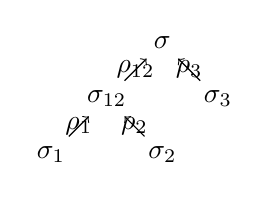
\begin{tikzpicture}
%\node(1) {$\sigma$};
%\node(2) [below right of=1] {$\sigma_{n}$};
%\node(3) [below left of=1] {$\sigma_{1\ldots n-1}$};
%\node(4) [below right of=3] {$\sigma_{n-1}$};
\node(5) {$\sigma$};
\node(6) [below right of=5] {$\sigma_{3}$};
\node(7) [below left of=5] {$\sigma_{12}$};
\node(8) [below right of=7] {$\sigma_2$};
\node(9) [below left of =7] {$\sigma_1$};
%\draw[loosely dotted] (6) to node {} (4);
%\draw[loosely dotted] (5) to node {} (3);
\draw[->] (9) to node {$\rho_1$} (7);
\draw[->] (7) to node {$\rho_{12}$} (5);
\draw[->] (6) to node {$\rho_{3}$} (5);
\draw[->] (8) to node {$\rho_2$} (7);
%\draw[->] (4) to node {$\rho_{n-1}$} (3);
%\draw[->] (3) to node {$\rho_{1\ldots n-1}$} (1);
%\draw[->] (2) to node {$\rho_{n}$} (1);
%\draw[->] (8) to [out=0, in=0, looseness=3] node [swap] {$i_2$} (1);
%\draw[->] (2) to [out=0, in=0, looseness=2] node  {$i_n$} (1);
%\draw[->] (4) to [out=0, in=0, looseness=3] node [swap] {$i_{n-1}$} (1);
%\draw[->] (6) to [out=0, in=0, looseness=3] node [swap] {$i_{n-1}$} (1);
\end{tikzpicture}
\]
The symbols $i_1$, $i_2$, and $i_3$ are function symbols with arity $\sigma_1\rightarrow \sigma$, $\sigma_2\rightarrow\sigma$, and $\sigma_3\rightarrow\sigma$, respectively.

We now turn to the proof.

\begin{proof}[Proof of Theorem \ref{mange}]
The following figure illustrates how our proof will be organized.
\begin{center}
\includegraphics{quineconjecture3revised.pdf}
\end{center}
Steps 1--3 define the theories $\widehat{T}_1,\ldots, \widehat{T}_{4}$, steps 4--6 define $T_1,\ldots, T_{4}$, and step 7 shows that $T_{4}$ and $\widehat{T}_{4}$ are logically equivalent.

\textbf{Step 1.} We begin by defining the theory $\widehat{T}_1$. For each sort $\sigma_j\in\Sigma$ we consider the following sentence.
\begin{align*}
\begin{aligned}
&\forall_\sigma y \left(q_{\sigma_j}(y)\leftrightarrow \exists_{\sigma_j} x(i_j(x)=y)\right) \\ &\qquad\land \forall_{\sigma_j} x_1\forall_{\sigma_j} x_2 (i_j(x_1)=i_j(x_2)\rightarrow x_1=x_2)
\end{aligned}
\tag{$\theta_{\sigma_j}$}
\end{align*}
The sentence $\theta_{\sigma_j}$ defines the symbols $\sigma_j$ and
$i_j$ as the subsort of ``things that are $q_{\sigma_j}$.'' The
auxiliary axioms $\phi_{\sigma_j}$ of $\widehat{T}$ guarantee that the
admissibility conditions for these definitions are satisfied. The
theory
$\widehat{T}_1=\widehat{T}\cup\{\theta_{\sigma_1},
\theta_{\sigma_2},\theta_{\sigma_3}\}$ is therefore a Morita extension
of $\widehat{T}$ to the signature
$\widehat{\Sigma}\cup\{\sigma_1,\sigma_2,\sigma_3, i_1,i_2,i_3\}$.

%We now show how the theory $\widehat{T}_1$ defines the new sorts $\sigma_{12}, \ldots, \sigma_{12,\ldots, n-1}$ and the function symbols $\rho_1, \rho_2, \ldots, \rho_{12\ldots n-1}, \rho_n$. 
\textbf{Step 2.} We now define the theories $\widehat{T}_2$ and $\widehat{T}_3$. Let $\theta_{\sigma_{12}}$ be a sentence that defines the symbols $\sigma_{12}, \rho_1, \rho_2$ as a coproduct sort. The theory $\widehat{T}_2=\widehat{T}_1\cup\{\theta_{\sigma_{12}}\}$ is clearly a Morita extension of $\widehat{T}_1$. 
%Likewise, the theory $\widehat{T}_1^1$ uses a sentence $\theta_{\sigma_{123}}$ to define the symbols $\sigma_{123}, \rho_{12}, \rho_3$ as a coproduct sort, resulting in another Morita extension $\widehat{T}_1^2=\widehat{T}\cup\{\theta_{\sigma_{12}}, \theta_{\sigma_{123}}\}$. 
%We repeat this process, at each step using the sentence $\theta_{\sigma_{1\ldots k}}$ to define the symbols $\sigma_{1\ldots k}$, $\rho_{1\ldots k-1}$, $\rho_k$ as coproduct sort, until we arrive at the theory 
%$$
%\widehat{T}_{n-1}=\widehat{T}_1\cup\{\theta_{\sigma_{12}}, \ldots, \theta_{\sigma_{1\ldots n-1}}\}
%$$
%in the signature $\widehat{\Sigma}\cup\{\sigma_1,\ldots, \sigma_n, i_1,\ldots, i_n\}\cup\{\sigma_{12},\ldots, \sigma_{12\ldots n-1}, \rho_1,\ldots, \rho_{n-1}\}$. One trivially sees that each $\widehat{T}_k$ that we have defined is a Morita extension of the theory $\widehat{T}_{k-1}$. 
%
We have yet to define the function symbols $\rho_{12}$ and $\rho_3$. The following two sentences define these symbols.
\begin{align*}
\tag{$\theta_{\rho_3}$}
&\forall_{\sigma_3} x \forall_\sigma y(\rho_3(x)=y\leftrightarrow i_3(x)=y)\\
%
&\forall_{\sigma_{12}} x \forall_\sigma y( \rho_{12}(x)=y\leftrightarrow \psi(x, y))
\tag{$\theta_{\rho_{12}}$}
\end{align*}
The sentence $\theta_{\rho_3}$ simply defines $\rho_3$ to be equal to the function $i_3$. For the sentence $\theta_{\rho_{12}}$, we define the formula $\psi(x,y)$ to be
%\begin{quote}
%Either (1) there is a $z$ such that $\rho_{n-1}(z)=z$ and $i_{n-1}(z)=y$ \textit{or} (2) there are $z_1$ and $z_2$ such that $\rho_{1\ldots n-2}(z_1)=x$, $\rho_{n-2}(z_2)=z_1$, and $i_{n-2}(z_2)=y$ \textit{or} \ldots \textit{or} ( 
%\end{quote}
\begin{align*}
&\exists_{\sigma_{1}} z_1 \big( \rho_{1}(z_1)=x\land i_{1}(z_1)=y\big)
\lor\exists_{\sigma_{2}} z_2\big( \rho_{2}(z_2)=x\land i_{2}(z_2)=y\big)
\end{align*}
We should take a moment here to understand the definition $\theta_{\rho_{12}}$. We want to define what the function $\rho_{12}$ does to an element $a$ of sort $\sigma_{12}$. Since the sort $\sigma_{12}$ is the coproduct of the sorts $\sigma_1$ and $\sigma_2$, the element $a$ must ``actually be'' of one of the sorts $\sigma_1$ or $\sigma_2$. (The disjuncts in the formula $\psi(x,y)$ correspond to these possibilities.) The definition $\theta_{\rho_{12}}$ stipulates that if $a$ is ``actually'' of sort $\sigma_j$, then the value of $\rho_{12}$ at $a$ is the same as the value of $i_j$ at $a$. One can verify that $\widehat{T}_{2}$ satisfies the admissibility conditions for $\theta_{\rho_3}$ and $\theta_{\rho_{12}}$, so the theory $\widehat{T}_3=\widehat{T}_{2}\cup\{\theta_{\rho_3}, \theta_{\rho_{12}}\}$ is a Morita extension of $\widehat{T}_{2}$ to the signature
$$
\widehat{\Sigma}\cup\{\sigma_1,\sigma_2, \sigma_3, \sigma_{12}, i_1,i_2, i_3, \rho_1, \rho_2,\rho_3, \rho_{12}\}
$$

\textbf{Step 3.} We now describe the $\Sigma^+$-theory $\widehat{T}_{4}$. This theory defines the predicates in the signature $\Sigma$. Let $p\in\Sigma$ be a predicate symbol of arity $\sigma_{j_1}\times\ldots\times\sigma_{j_m}$. We consider the following sentence.
\begin{align*}
\tag{$\theta_{p}$}
\forall_{\sigma_{j_1}} x_1\ldots \forall_{\sigma_{j_m}} x_m\left(p(x_1,\ldots, x_m)\leftrightarrow q_{p}(i_{j_1}(x_1),\ldots, i_{j_m}(x_m))\right)
\end{align*}
The theory $\widehat{T}_{4}=\widehat{T}_3\cup\{\theta_{p}:p\in\Sigma\}$ is therefore a Morita extension of $\widehat{T}_3$ to the signature $\Sigma^+$.

\textbf{Step 4.} We turn to the left-hand side of our organizational figure and define the theories $T_1$ and $T_{2}$. We proceed in an analogous manner to the first part of Step 2. The theory $T_1=T\cup\{\theta_{\sigma_{12}}\}$ is a Morita extension of $T$ to the signature $\Sigma\cup\{\sigma_{12}, \rho_1,\rho_2\}$. Now let $\theta_\sigma$ be the sentence that defines the symbols $\sigma, \rho_{12}, \rho_3$ as a coproduct sort. The theory $T_{2}=T_{1}\cup\{\theta_{\sigma}\}$ is a Morita extension of $T_{1}$ to the signature $\Sigma\cup\{\sigma_{12}, \sigma, \rho_1, \rho_2, \rho_3, \rho_{12}\}$.

\textbf{Step 5.} This step defines the function symbols $i_1$, $i_2$, and $i_3$. We consider the following sentences.
\begin{align*}
\tag{$\theta_{i_3}$}
&\forall_{\sigma_3} x_3 \forall_{\sigma} y(i_3(x_3)=y\leftrightarrow \rho_3(x_3)=y)\\
\tag{$\theta_{i_{2}}$}
%
&\forall_{\sigma_{2}}x_{2} \forall_{\sigma} y\big(i_{2}(x_{2})=y\leftrightarrow\exists_{\sigma_{12}} z( \rho_{2}(x_{2})=z\land\rho_{12}(z)=y)\big)\\
%
&\forall_{\sigma_1}x_1\forall_{\sigma}y\big(i_1(x_1)=y\leftrightarrow\exists_{\sigma_{12}} z(\rho_1(x_1)=z\land\rho_{12}(z)=y)\big)
\tag{$\theta_{i_1}$}
\end{align*}
The sentence $\theta_{i_3}$ defines the function symbol $i_3$ to be equal to $\rho_3$. The sentence $\theta_{i_{2}}$ defines the function symbol $i_{2}$ to be equal to the composition ``$\rho_{12}\circ\rho_{2}$.'' Likewise, the sentence $\theta_{i_{1}}$ defines the function symbol $i_{1}$ to be ``$\rho_{12}\circ\rho_{1}$.'' The theory $T_3=T_{2}\cup\{\theta_{i_1},\theta_{i_2}, \theta_{i_3}\}$
is a Morita extension of $T_{2}$ to the signature $\Sigma\cup\{\sigma_{12}, \sigma, \rho_1, \rho_2, \rho_3, \rho_{12}, i_1, i_2, i_3\}$.

\textbf{Step 6.} We still need to define the predicate symbols in $\widehat{\Sigma}$. Let $\sigma_j\in\Sigma$ be a sort symbol and $p\in\Sigma$ a predicate symbol of arity $\sigma_{j_1}\times\ldots\times\sigma_{j_m}$. We consider the following sentences.
\begin{align*}
&\begin{aligned}
\forall_{\sigma} y(q_{\sigma_j}(y)\leftrightarrow\exists_{\sigma_j} x(i_j(x)=y))
\end{aligned}
\tag{$\theta_{q_{\sigma_j}}$}\\
%
&\begin{aligned}
\forall_\sigma y_1\ldots\forall_\sigma y_m\big(q_{p}(y_1,\ldots, y_m)\leftrightarrow&\exists_{\sigma_{j_1}} x_1\ldots\exists_{\sigma_{j_m}} x_m(i_{j_1}(x_1)=y_1\land\ldots\\&\land i_{j_m}(x_m)=y_m\land p(x_1,\ldots, x_m))\big)
\end{aligned}
\tag{$\theta_{q_{p}}$}
\end{align*}
These sentences define the predicates $q_{\sigma_j}\in\widehat{\Sigma}$ and $q_p\in\widehat{\Sigma}$. One can verify that $T_3$ satisfies the admissibility conditions for the definitions $\theta_{q_{\sigma_j}}$. And therefore the theory $T_{4}=T_3\cup\{\theta_{q_{\sigma_1}}, \theta_{q_{\sigma_2}}, \theta_{q_{\sigma_3}}\}\cup\{\theta_{q_{p}}: p\in\Sigma\}$ is a Morita extension of $T_3$ to the signature $\Sigma^+$.

\textbf{Step 7.} It only remains to show that the $\Sigma^+$-theories
$T_{4}$ and $\widehat{T}_{4}$ are logically equivalent. One can verify
by induction on the complexity of $\psi$ that
\begin{equation}
  T_{4}\vdash\psi\leftrightarrow\widehat{\psi}\quad \text{and} \quad \widehat{T}_{4}\vdash\psi\leftrightarrow\widehat{\psi}.
\label{step7}
\end{equation}
for every $\Sigma$-sentence $\psi$. One then uses \eqref{step7} to
show that $T_{4}$ and $\widehat{T}_{4}$ are logically equivalent. The
argument involves a number of cases, but since each case is
straightforward we leave them to the reader to verify. The theories
$T_{4}$ and $\widehat{T}_{4}$ are logically equivalent, which implies
that $T$ and $\widehat{T}$ are Morita equivalent.
\end{proof}

Theorem \ref{mange} shows that Quine was right to say that every
many-sorted theory is equivalent to a single-sorted theory.  But what
is the philosophical significance of this result?  There is no doubt
about what Quine thought about its significance.  He claimed that
many-sorted logic was at best inessential, and at worst, a misleading
guide to the structure of knowledge and/or reality.  Whether he was
right or wrong, Quine has been almost single-handedly responsible for
the fact that many-sorted logic has not figured in the standard
curriculum for analytic philosophy students.  Indeed, far more
analytic philosophers are familiar with modal logic than are with
many-sorted logic (based on our anecdotal evidence from teaching,
reading journals, and talking with other philosophers).  We hope that
our efforts in this book go some way to fixing this problematic
situation.


\section{Translation generalized} \label{trans-g}

In the previous chapters, we've talked about various notions of a
``translation'' between theories.  Of course, we did not find the
definition of translation written on tablets of stone; nor did we have
a Platonic vision of the one true form of a translation.  No, we found
Quine's definition in the literature, and it works quite well for some
purposes, but it's also quite restrictive.  In particular, Quine's
notions of reconstrual and translation are not general enough to
capture some well-known cases of translations between the theories of
pure mathematics.

\begin{enumerate}
\item In the 19th century, the German mathematician Leopold Kronecker
  is reported to have said, ``God made the integers, all else is the
  work of man.''  In more prosaic terms, talk about higher number
  systems --- such as rational, real, and complex numbers --- can be
  {\it reduced} to talk about integers.  However, to effect such a
  reduction, one must treat each rational number as a pair of integers
  --- or, more accurately, as an equivalence class of pairs of
  integers.  Similarly, to reduce the complex numbers to the real
  numbers, one must treat a complex number as a pair of real numbers,
  viz.\ the real and imaginary parts of the complex number.
\item Now for a more controversial example, which we will take up at
  greater length in Section \ref{go-geometry}.  There are different
  ways that one can write down axioms for Euclidean geometry.  In one
  axiomatization, the basic objects are points; and in another
  axiomatization, the basic objects are lines.  Is there a sense in
  which these two axiomatized theories could both be Euclidean
  geometry, in particular, that they could be equivalent?  The answer
  is Yes, but only if one allows translations that take a single
  variable of the first theory to a pair of variables of the second
  theory.  In particular, a line needs to be treated as an equivalence
  class of pairs of points; and a point needs to be treated as a pair
  of intersecting lines.
\end{enumerate}

In the previous chapter, we required that a formula $p(x)$ of $\Sigma$
be translated to a formula $\vp (x)$ of $\Sigma '$.  There's one
particular part of this recipe that seems questionable: why would the
same variable $x$ occur in both formulas?  In general, why suppose
that two signatures $\Sigma$ and $\Sigma '$ should share the same
variables in common?  It's not like variables have some
``trans-theoretical'' meaning that must be preserved by any reasonable
translation.

But how then can variables be reconstrued in moving from one theory to
another?  One natural proposal would be to include in a reconstrual a
mapping from variables of $\Sigma$ to variables of $\Sigma '$, i.e.\ a
function that assigns a variable of $\Sigma '$ to each variable of
$\Sigma$.  Even so, it's a non-trivial question whether there is an
in-principle reason that a single variable in $\Sigma$ must be
reconstrued as a single variable in $\Sigma '$.  Perhaps one theorist
uses several variables to do the work that the other theorist manages
to do with a single variable.  Such cases are not hard to find in the
sciences --- for example, when the objects of one mathematical theory
are reconstrued as ``logical constructions'' of objects in another
mathematical theory.

Let's proceed then under the assumption that a single variable in one
language could be reconstrued in terms of multiple variables in
another language.  Thus, a reconstrual, in the formal sense, should
include a function that matches variables of the signature $\Sigma$ to
$n$-tuples of variables of the signature $\Sigma'$.

Consider again the case of reconstruing rational numbers (i.e.\
fractions) as pairs of integers.  Of course, not {\it every} pair of
integers gives a well-defined fraction.  For example, there is no
fraction of the form $\frac{1}{0}$.  In that case, the ``integer
theorist'' doesn't think of the domain of fractions as consisting of
all pairs of integers; rather, she thinks of that domain as consisting
of pairs of integers where the second entry is non-zero.  To capture
this nuance --- the restriction of the domain of quantification --- we
stipulate that a reconstrual $F$ includes a formula $D$ of the target
language $\Sigma '$.  In the running example, the formula $D$ could be
given by
\[ D(x,y) \: \equiv \: (x=x)\wedge (y\neq 0) .\] The integer theorist
can then use the formula $D$ to restrict her quantifiers to the domain
of well-defined fractions.

Finally, and most controversially, let's consider how we might
reconstrue the equality relation $=$ of the domain theory $T$ as a
relation of the target theory $T'$.  (Our choice here will prove to be
controversial when we show that it yields a positive verdict in favor
of quantifier variance.  See Example \ref{ex:nihil}.)  Recall that the
single variables $x$ and $y$ will typically be reconstrued as
$n$-tuples of variables $\vec{x}$ and $\vec{y}$.  In that case, how
should we reconstrue the formula $x=y$?  One might naturally propose
that $x=y$ be reconstrued as the formula
\begin{equation} (x_1=y_1)\wedge (x_2=y_2)\wedge \cdots \wedge
  (x_n=y_n) .\label{simple} \end{equation} But here we need to think a
bit harder about how and why variables of $\Sigma$ are encoded as
variables of $\Sigma '$.  For this, let's consider again the example
of rational numbers being reduced to integers:

Consider a formula $x=y$ in the theory of rational numbers.  To the
``integer theorist,'' the variables $x$ and $y$ really represent
complex entities, namely fractions.  What's more, to say that two
fractions $\frac{x_1}{x_2}$ and $\frac{y_1}{y_2}$ are equal does not
mean that $x_1=y_1$ and $x_2=y_2$.  Rather,
$\frac{x_1}{x_2}=\frac{y_1}{y_2}$ means that
$x_1\times y_2=y_1\times x_2$.  In other words, the formula $x=y$ of
the language of the rational numbers is reconstrued as the formula
\begin{equation} x_1\times y_2=y_1\times x_2
  ,\label{foo} \end{equation} in the language of the integers, where
$\times$ is the multiplication operation.

This example suggests that we might not always want the formula $x=y$
to be reconstrued as Eqn.\ \ref{simple}.  Instead, we might prefer to
reconstrue $x=y$ as some other $\Sigma '$ formula
$E(x_1,\dots ,x_n;y_1,\dots ,y_n)$.  Of course, not everything goes:
$E$ will need to perform the same functions in the theory $T'$ that
the formula $x=y$ performs in the theory $T$.  In particular, we will
require that $E$ be an equivalence relation relative to the theory
$T'$.

We're now ready to consider ways in which the elements of one
signature $\Sigma$ can be reconstrued as syntactic structures built
from a second signature $\Sigma '$.  (We include here the case where
$\Sigma '=\Sigma$.  In that case, we will be considering substitutions
and permutations of notation.)  The case of relation symbols is
relatively easy: an $m$-ary relation symbol $r$ of $\Sigma$ should
correspond to a formula $F(r)$ of $\Sigma '$ with $mn$ free variables.
To be even more precise, it's the relation symbol $r$ and an $n$-tuple
of variables $x_1,\dots ,x_n$ that corresponds to some particular
formula $F(r)$ of $\Sigma '$, and we require that
$FV(F(r))=\{ \vec{x}_1,\dots ,\vec{x}_n \}$.

We will need to proceed with more caution for the function symbols in
the signature $\Sigma$.  The question at issue is: which syntactic
structures over $\Sigma '$ are the proper targets for a reconstrual of
the function symbols in $\Sigma$?  To say that the target must be
another function symbol is too restrictive.  Indeed, there's a
well-known ``theorem'' which says that every first-order theory is
equivalent to a theory that uses only relation symbols.  (The reason
that ``theorem'' is placed in quotes here is because the result cannot
be proven with mathematical rigor until the word ``equivalent'' is
defined with mathematical rigor.)  The trick to proving that theorem
is to reconstrue each function symbol $f$ as a relation
\[ p_f(x_1,\dots ,x_m,y) \: \equiv \: (f(x_1,\dots ,x_m) = y) ,\] and
then to add axioms saying that $p_f$ relates each $m$-tuple
$x_1,\dots ,x_m$ to a unique output $y$.  If we are to be able to
validate such a result (which is intuitively correct), then we ought
to permit function symbols of $\Sigma$ to be reconstrued as formulas
of $\Sigma '$.  We will deal with this issue by analogy with the way
we dealt with relation symbols above: a function symbol $f$ of
$\Sigma$ and $m+1$ variables $x_1,\dots ,x_n,y$ of $\Sigma$ ought to
correspond to a formula $(Ff)(\vec{x}_1,\dots ,\vec{x}_n,\vec{y})$ of
$\Sigma '$.


  %% TO DO: straighten out notation for collection of sorts

  In order to define a more general notion of a translation, the key
  is to allow a single sort $\sigma$ of $\Sigma$ to be mapped to a
  sequence of sorts of $\Sigma '$, including the case of repetitions
  of a single sort.  The idea, in short, is to encode a single
  variable (or quantifier) in $\Sigma$ by means of several variables
  (or quantifiers) in $\Sigma '$.  In order to make this idea more
  clear, it will help to give a precise definition of the monoid of
  finite sequences from a set $S$.

  \begin{defn} For a set $S$, we let $S^*$ denote the \emph{free
      monoid} on $S$, which is uniquely defined by the following
    universal property: there is a function $\eta _S:S\to S^*$, and
    for any monoid $A$, and function $f:S\to A$, there is a unique
    monoid morphism $f^*:S^*\to A$ such that $f^*\circ\eta _S=f$.
    Concretely speaking, $S^*$ can be constructed as the set
  \[ S \amalg (S\times S)\amalg (S\times S\times S) \amalg \cdots ,\]
  where $\eta _S:S\to S^*$ is the first coprojection.  In this case,
  given $f:S\to A$, $f^*:S^*\to A$ is the function
  \[ f^*(s_1,\dots ,s_n) \: = \: f(s_1)\circ \cdots\circ f(s_n) ,\]
  where $\circ$ is the monoid operation on $A$.  \end{defn}

\begin{defn} \label{gro} Let $\Sigma$ and $\Sigma '$ be many-sorted
  signatures with sets of sorts $S$ and $S'$ respectively.  A
  generalized \emph{reconstrual} $F:\Sigma \to \Sigma '$ consists of:
  \begin{enumerate}
  \item A function $F:S\to (S')^*$.  That is, $F$ maps the sorts of
    $\Sigma$ to non-empty sequences of sorts of $S'$.  For each
    $\sigma\in S$, let $d(\sigma )$ be the length of the sequence
    $F(\sigma )$.  We call $d:S\to\7N$ the \emph{dimension function}
    of $F$.
  \item A corresponding function
    $x\mapsto \vec{x}=x_1,\dots ,x_{d(\sigma )}$ from
    $\Sigma$-variables to sequences of $\Sigma '$-variables, such that
    $x_i:F(\sigma )_i$.  We require that if $x\not\equiv y$, then the
    sequences $\vec{x}$ and $\vec{y}$ have no overlap.
  \item A function $D$ from $\Sigma$-variables to $\Sigma '$-formulas.
    We call $D_x$ a \emph{domain formula}.  We require the map
    $x\mapsto D_x$ to be natural in the following sense: if $y$ is of
    the same sort as $x$, then $D_y=D_x[\vec{y}/\vec{x}]$.
  \item A function $F$ that takes a relation symbol $p$ of $\Sigma$,
    and a suitable context $x_1,\dots ,x_n$ of variables from
    $\Sigma$, and yields a formula $(Fp)(\vec{x}_1,\dots ,\vec{x}_n)$
    of $\Sigma '$.  We again require this map to be natural in the
    sense that
    \[ (Fp)(\vec{y}_1,\dots ,\vec{y}_n) \: = \: (Fp)(\vec{x}_1,\dots
      ,\vec{x}_n)[\vec{y}_1,\dots ,\vec{y}_n/\vec{x}_1,\dots
      ,\vec{x}_n] .\] \end{enumerate}
\end{defn}


%    \item For each sort symbol $\sigma\in S$, a natural map $E^\sigma$
%     from pairs of variables of sort $\sigma$ to a formula with pairs
%     of variables of sort $F(\sigma )$.  Thus, $E^\sigma_{x,y}$ is a
%     $\Sigma '$-formula with free variables
%     $\vec{x}=x_1,\dots ,x_{d(\sigma )}$ and
%     $\vec{y}=y_1,\dots ,y_{d(\sigma )}$, where $d(\sigma )$ is the
%     length of the sequence $F(\sigma )$.  To say that $E_\sigma$ is
%     natural means that
%     $E_\sigma (v,w)=E_\sigma (x,y)[\vec{v},\vec{w}/\vec{x},\vec{y}]$,
%     or in diagrammatic form:
%     \[ \begin{tikzcd} v,w\arrow{r}{[x,y/v,w]} \arrow{d} & x,y \arrow{d} \\
%         E_\sigma (v,w) \arrow{r}{[\vec{x},\vec{y}/\vec{v},\vec{w}]} &
%         E_\sigma (x,y) \end{tikzcd} \] We write $D_\sigma (x)$ for
%     $E _\sigma (x,x)$, and call $D_\sigma (x)$ a \emph{domain
%       formula}.  When no confusion can result, we drop the $\sigma$
%     from $E_\sigma$ and $D_\sigma$.
%   \item We require that each $E(x,y)$ is a non-empty, partial
%     equivalence relation in the sense that
%     \[ \vdash \exists \vec{x} E(x,x) \qquad E(x,y)\vdash E(y,x) \qquad
%       E(x,y)\wedge E(y,z)\vdash E(x,z) \] Thus, $E(x,y)$ is a full
%     equivalence relation on domain $D(x)$.
   
% \item For each function symbol $f\in\Sigma$, we define $Ff$ as a
%   natural map from contexts for $f$ to $\Sigma '$-formulas.  More
%   precisely: if $x_1,\dots ,x_n$ is an appropriate context for $f$,
%   and $y$ is of the output sort for $f$, then $F(f)(x_1,\dots ,x_n,y)$
%   is a $\Sigma _2$-formula with free variables
%   $\vec{x}_1,\dots ,\vec{x}_n,\vec{y}$ of the appropriate sorts.  We
%   require that $Ff$ is natural under substitution of variables, is
%   compatible with the equivalence relation $E(\vec{x},\vec{y})$, and
%   is a functional relation from $D(\vec{x})$ to $D(\vec{y})$, relative
%   to $E(\vec{x},\vec{y})$:
%   \[ (Ff)(x,y)\wedge (Ff)(x,z) \:\vdash \:E(\vec{y},\vec{z}) \]
%   \[ D(\vec{x}) \:\vdash \: \exists\vec{y}(Ff)(x,y) \]
% \end{enumerate}
% \end{defn}

% This definition may seem too complicated for any practical use.
% However, it's actually fairly easy to define legitimate reconstruals
% without thinking too hard about all of these conditions.  In short, if
% $\sigma$ goes to a sequence $\sigma _1,\dots ,\sigma _n$, then we need
% to map equality on $\sigma$ to some equivalence relation $E$ on
% $\sigma _1,\dots ,\sigma _n$.  Then for each relation symbol $p$ of
% $\Sigma$, we define $(Fp)(x_1,\dots ,x_n)$ to be a $\Sigma '$-formula
% $\phi (\vec{x}_1,\dots ,\vec{x}_n)$, with the implicit understanding
% then that $(Fp)(y_1,\dots ,y_n)$ is the formula
% $\phi (\vec{y}_1,\dots ,\vec{y}_n)$ that results from uniform
% substitution.  Function symbols are a bit more tricky, since we map
% them not to function symbols, but to relation symbols.  However, given
% a function symbol $f$ of $\Sigma$, we map $f(x_1,\dots ,x_n)=y$ to a
% relation symbol $\phi (\vec{x}_1,\dots ,\vec{x}_n,\vec{y})$, again
% with the understanding that substitutions on the domain formula
% correspond to appropriate substitutions on the codomain formula.

A reconstrual $F$ naturally extends to a map from $\Sigma$-formulas to
$\Sigma '$-formulas.  We define this extension, also called $F$, so
that for any $\Sigma$-formula $\phi$, with $x$ free in $\phi$, the
following two constraints are satisfied:
\[ F(\phi )\:\vdash \: D(\vec{x}) ,\qquad \qquad F(\phi [y/x]) \: = \:
  F(\phi )[\vec{y}/\vec{x}] , \] The first restriction is not
technically necessary --- it is simply a convenient way to ignore
whatever the formula $F(\phi )$ says about things outside of the
domain $D(\vec{x})$.  (This apparently minor issue plays a significant
role in Quine's argument for the dispensability of many-sorted logic.
See \ref{qboom}.)  Accordingly, for a relation symbol $p$ of $\Sigma$,
we first redefine $(Fp)(\vec{x}_1,\dots ,\vec{x}_n)$ by conjoining
with $D(\vec{x}_1)\wedge\cdots\wedge D(\vec{x}_n)$.  (We could have
also have included this condition in the very definition of a
reconstrual.)  The extension of $F$ proceeds as
follows: \begin{itemize}
\item Let $F(\phi\wedge \psi )=F(\phi )\wedge F(\psi )$, and let
  $F(\phi\vee\psi )=F(\phi )\vee F(\psi )$. 
\item Let
  $F(\neg \phi ) =\neg F(\phi )\wedge D(\vec{x}_1)\wedge\cdots\wedge
  D(\vec{x}_n)$, where $x_1,\dots ,x_n$ are all the free variables
  that occur in $\phi$.
\item Let $F(\phi\to\psi )=F(\neg\phi )\vee F(\psi )$.
\item Let
  $F(\exists x\phi )=\exists \vec{x}(D(\vec{x})\wedge F(\phi ))$.
\item Let $F(\forall x\phi )=\forall \vec{x}(D(\vec{x})\to F(\phi ))$.
\end{itemize}
  
\begin{defn} Let $F:\Sigma \to\Sigma '$ be a reconstrual.  We say that
  $F$ is a \emph{translation} of $T$ into $T'$ just in case: for every
  $\Sigma$-sentence $\phi$: if $T\vdash\phi$ then $T'\vdash F(\phi )$.
  In this case, we write $F:T\to T'$.  In the case that $\Sigma$ has a
  single sort $\sigma$, we say that $F$ is a $d(\sigma )$-dimensional
  translation.  \end{defn}

The definition of a translation allows us to handle the case where the
domain signature $\Sigma$ has equality relations and function symbols.
In particular, for each theory $T$ in $\Sigma$, we explicitly include
the following axioms:
\begin{itemize}
\item The equality introduction axioms: $\vdash x=_\sigma x$.
\item The equality elimination axioms:
  $\phi (x),(x=_\sigma y)\vdash \phi (y)$, for each atomic or negated
  atomic formula $\phi$ of $\Sigma$.
\end{itemize}
As usual, these axioms together entail that $=_\sigma$ is an
equivalence relation.  Thus, if $F:T\to T'$ is a translation, then
$F(=_\sigma )(\vec{x},\vec{y})$ is an equivalence relation on domain
$D(\vec{x})$.  We abbreviate this relation by
$E_\sigma (\vec{x},\vec{y})$, or when no confusion can result, simply
as $E(\vec{x},\vec{y})$.  In this case, for each relation symbol $p$
of $\Sigma$, 
\[ T',(Fp)(\vec{x}), E(\vec{x},\vec{y})\:\vdash \: (Fp)(\vec{y}) .\]
Roughly speaking, the predicate $Fp$ has to be compatible with the
equivalence relation $E$: it holds of something iff it holds of
everything $E$-equivalent to that thing.  Equivalently, the extension
of $Fp$ is a union of $E$-equivalence classes.

Now suppose that $\Sigma$ contains a constant symbol $c$.  Then,
choosing a variable $x$ of the same sort, $c=x$ is a unary formula,
and $F(c=x)$ is a formula $\phi (\vec{x})$.  The theory $T$ entails
that the formula $c=x$ is uniquely satisfied.  Hence, if $F:T\to T'$
is a translation, then $T'$ entails that $\phi (\vec{x})$ is uniquely
satisfied --- relative to the equivalence relation $E$.  In short $T'$
implies both $\exists \vec{x}(D_x\wedge \phi (\vec{x}))$ and
$\phi (\vec{x})\wedge \phi (\vec{y})\to E(\vec{x},\vec{y})$.
Intuitively speaking, this means that the extension of
$\phi (\vec{x})$ is a single $E$-equivalence class.

Similar reasoning applies to the case of any function symbol $f$ of
$\Sigma$.  The $\Sigma$-formula $f(x_1,\dots ,x_n)=y$ is reconstrued
as some $\Sigma '$-formula
$\phi (\vec{x}_1,\dots ,\vec{x}_n,\vec{y})$.  If $F:T\to T'$ is a
translation, then $T'$ entails that $\phi$ is a functional relation
relative to $E$-equivalence.  What this means intuitively is that
$\phi$ is a function from $E$-equivalence classes to $E$-equivalence
classes.

%%% Examples

\begin{example}[Quantifier variance] \label{go-qv} We now undertake an
  extended discussion of an example that is near and dear to
  metaphysicians: the debate between mereological universalism and
  nihilism.  To keep the technicalities to a bare minimum, we will
  consider a dispute over whether the composite of two things exists.
  Suppose that the parties to the dispute are are named Niels the
  Nihilist and Mette the Mereological Universalist.  Niels says that
  there are exactly two things, whereas Mette says that there are
  exactly three things, one of which is composed of the other two.

  Now, we press Niels and Mette to regiment their theories, and here's
  what they come up with.  Niels has a signature $\Sigma$, which is
  empty, very much in line with his predilection for desert
  landscapes.  Niels' theory has a single axiom, ``there are exactly
  two things.''  Mette has a signature $\Sigma '$ with a binary
  relation symbol $p$ that she'll use to express the parthood
  relation.  Mette's theory $T'$ says that $p$ is a strict partial
  order, that there are exactly two atoms, and exactly one thing above
  those two atoms.  Note that Mette can define an open formula in
  $\Sigma '$
  \[ a(x) \: \equiv \: \neg \exists y\, p(y,x) ,\] which intuitively
  expresses the claim that $x$ is an atom.

  At the turn of the 21st century, metaphysicians were engaged in a
  fierce debate about whether Niels or Mette has a better theory.
  Then some other philosophers, such as Eli Hirsch, said, ``stop
  arguing --- it's merely a verbal dispute, like an argument about
  whether there are six roses or half a dozen roses''
  \citep[see][]{chalmers,hirschbog}.  These other philosophers espouse
  a position known as \emph{quantifier variance}.  One clear
  explication of quantifier variance would be to say that Niels and
  Mette's theories are \emph{equivalent}.  So are they equivalent or
  not?  The answer to this question depends (unsurprisingly) on the
  standard of equivalence that we adopt.  For example, it is easy to
  see that Niels and Mette's theories are not strictly
  intertranslatable in the sense of Defn \ref{def:itrans}.  However,
  we will now see that Niels and Mette's theories are
  intertranslatable in the weaker sense described in Defn
  \ref{def:weak}.

  It seems clear that Mette can make sense of Niels' theory --- in
  particular, that she can identify Niels' quantifier as a restriction
  of her own.  The idea that Mette can ``make sense of Niels' theory''
  can be cashed out formally as saying that Niels' theory can be
  translated into Mette's theory.  Intuitively speaking, for any
  sentence $\phi$ asserted by Niels, there is a corresponding sentence
  $\phi ^*$ asserted by Mette.  For example, when Niels says
  \begin{quote} There are exactly two things,
  \end{quote}
  Mette can charitably interpret him as saying, 
  \begin{quote}
    There are exactly two atoms. \end{quote}

  Now we show that there is indeed a translation $F:T\to T'$, where
  $T$ is Niels' theory, and $T'$ is Mette's theory.  Here Niels and
  Mette's theories are single-sorted, and we define $F$ to be a
  one-dimensional reconstrual.  We define the domain formula as
  $D_F(x)=a(x)$, and we translate Niels' equality relation as Mette's
  equality relation restricted to $D_F$.

  Let's just check that $F$ is indeed a translation.  While a general
  argument is not difficult, let's focus on Niels' controversial
  claim $\phi$: that there are {\it at most two} objects in the domain: 
  \[ \phi \:\equiv \: \forall x\forall y\forall z((x=y)\vee (x=z)\vee
    (y=z)) .\] The reconstrual $F$ takes $x=y$ to the formula
  $a(x')\wedge a(y')\wedge (x'=y')$, and hence $F(\phi )$ is the
  uncontroversially true statement that there are at most two atoms.
  Of course, Mette agrees with that claim, and so $F:T\to T'$ is a
  translation of Niels' theory into Mette's.

  Indeed, $F$ is a particularly nice translation: it's conservative,
  in the sense that if $T'\vdash F(\phi )$ then $T\vdash \phi$.  Thus,
  not only does Mette affirm everything that Niels says about atoms,
  Niels also affirms everything that Mette says about atoms.  Thus,
  there is a precise sense in which Niels' theory is simply a
  ``sub-theory'' of Mette's theory.  They are in complete agreement
  relative to their shared language, and Mette simply has a larger
  vocabulary than Niels.

  The existence of the translation $F:T\to T'$ comes as no surprise.
  But what about the other way around?  Can Niels be as charitable to
  Mette as she has been to him?  Can he find a way to affirm {\it
    everything} that she says?  The answer to that question is far
  from clear.  For example, Mette says things like, ``$x$ is a
  composite of $y$ and $z$.''  How in the world could Niels make sense
  of that claim?  How in the world could Niels say, ``what Mette says
  here is perfectly correct, if only understood in the proper way''?
  Similarly, Mette says that ``there are more than two things.''  How
  in the world could Niels validate such a claim?

  We will now see that Niels can indeed charitably interpret, and
  endorse, all of Mette's assertions.  Indeed, Niels needs only think
  of Mette's notion of ``a thing'' as corresponding to what he means
  by ``a pair of things'' --- as long as two pairs are considered to
  be ``the same'' when they are permutations of each other.

  More precisely, consider a $2$-dimensional reconstrual
  $G:\Sigma '\to \Sigma$ which encodes a $\Sigma '$-variable $x$ as a
  pair $x_1,x_2$ of $\Sigma$-variables.  Define $D_G(x_1,x_2)$ to be
  the formula $(x_1=x_1)\wedge (x_2=x_2)$ that holds for all pairs
  $\langle x_1,x_2\rangle$.  Define $E_G(x_1,x_2,y_1,y_2)$ to be the
  relation that holds between $\langle x_1,x_2\rangle$ and
  $\langle y_1,y_2\rangle$ just in case one is a permutation of the
  other.  That is,
  \[ E_G(x_1,x_2,y_1,y_2) \: \equiv \: (x_1=y_1\wedge x_2=y_2)\vee
    (x_1=y_2\wedge x_2=y_1 ) .\] Clearly $T$ entails that $E_G$ is an
  equivalence relation.

  The signature $\Sigma '$ consists of a single binary relation symbol
  $p$.  Since $G$ is $2$-dimensional, $Gp$ must be defined to be a
  four-place relation in $\Sigma$.  Here is the intuitive idea behind
  our definition of $Gp$: we will simulate atoms of Mette's theory by
  means of diagonal pairs, i.e.\ pairs of the form
  $\langle x,x\rangle$.  We then say that $Gp$ holds precisely between
  pairs when the first is diagonal, the second is not, and the first
  has a term in common with the second.  More precisely,
  \[ (Gp)(x_1,x_2,y_1,y_2) \: \equiv \: (x_1=x_2)\wedge (y_1\neq y_2
    )\wedge (x_1=y_1\vee x_1=y_2) .\] Recall that $a(x)$ is the
  formula of $\Sigma '$ which says that $x$ is an atom.  We claim now
  that the translation $G(a(x))$ of $a(x)$ holds precisely for the
  pairs on the diagonal.  That is,
  \[ T\:\vdash \: G(a)(x_1,x_2)\leftrightarrow (x_1=x_2 ) .\] We argue
  by reductio ad absurdum.  (Here we use the notion of a model, which
  will first be introduced in the next chapter.  Hopefully the
  intuition here is clear.)  First, if
  \[ T\:\not\vdash \: G(a)(x_1,x_2)\rightarrow (x_1=x_2 ), \] then
  there is a model $M$ of $T$, and two distinct objects $c,d$ of $M$
  such that $M\models G(a)(c,d)$.  That means that
  \[ M\models \neg \exists y\exists z\, G(p)(y,z,c,d) .\] But clearly
  $M\models G(p)(c,c,c,d)$, a contradiction.  To prove the other
  direction it will suffice to show that for any model $M$ of $T$, and
  for any $c\in M$, we have $M\models G(a)(c,c)$.  Recalling that $T$
  only has one model, namely a model with two objects, the result
  easily follows.
  
  When Mette the Mereologist says that there are more than two things,
  Niels the Nihilist understands her as saying that there are more
  than two pairs of things.  Of course, Niels agrees with that claim.
  In fact, it's not hard to see that, under this interpretation, Niels
  affirms everything that Mette says. \end{example}

\begin{disc} We've shown that Niels' theory can be translated into
  Mette's, and vice versa.  Granting that this is a good notion of
  ``translation,'' does it follow that these two theories are
  equivalent?  In short, No.  Recall the simpler case of propositional
  theories.  For example, let $\Sigma = \{ p_0,p_1,\dots \}$, let $T$
  be the empty theory in $\Sigma$, and let $T'$ be the theory with
  axioms $p_0\vdash p_1,p_0\vdash p_2,\dots $.  Then there are
  translations $f:T\to T'$ and $g:T'\to T$, but $T$ and $T'$ are not
  equivalent theories.  In general, mutual translatability is not
  sufficient for equivalence.  Nonetheless, we will soon see (Example
  \ref{ex:nihil}) that there is a precise sense in which Niels and
  Mette's theories are indeed equivalent.  \hfill \qed
\end{disc}

We are now ready to prove a generalized version of the
\textbf{substitution theorem}.  In its simplest form, the substitution
theorem says a valid derivation $\vp _1,\dots ,\vp_n\vdash \psi$ is
preserved under uniform substitution of the non-logical symbols in
$\phi _1,\dots ,\phi _n$ and $\psi$.  For example, from a valid
derivation of $\exists x(p(x)\wedge q(x))\vdash \exists x p(x)$,
substitution of $\forall y(r(y,z)$ for $p(x)$ yields a valid
derivation of
\[ \exists z(\forall yr(y,z)\wedge q(z)) \: \vdash \: \exists z\forall
  yr(y,z) .\] However, we need to be careful in describing what counts
as a legitimate ``substitution instance'' of a formula.  Let's test
our intuitions against an example.

\begin{example} Let $\Sigma$ be a single-sorted signature with
  equality, but no other symbols.  Let $\Sigma '$ be a single-sorted
  signature with equality, and one other monadic predicate $D(x)$.  We
  define a 1-dimensional reconstrual $F:\Sigma\to\Sigma '$ by taking
  $D(x)$ to be the domain formula, and by taking $E(x,y)$ to be
  equality in $\Sigma '$.  We will see now that the substitution
  theorem does {\it not} hold in the form: if $\phi\vdash\psi$ then
  $F(\phi)\vdash F(\psi )$.

  In $\Sigma$ we have $x\neq y \vdash \exists z(x\neq z)$.  Since $F$
  translates equality in $\Sigma$ to equality in $\Sigma '$, we have
  $F(x\neq y)\equiv (x\neq y)$.  Furthermore, $F(\exists z(x\neq z))$
  is the relativized formula $\exists z(D(z)\wedge x\neq z)$.  But
  $x\neq y$ does not imply there there is a $z$ such that $D(z)$ and
  $x\neq z$.  For example, in the domain $\{ a,b\}$, if the extension
  of $D$ is $\{ a\}$, then $a\neq b$, but not
  $\exists z(D(z)\wedge a\neq z)$.  Thus, the substitution theorem
  does {\it not} hold in the form: if $\phi\vdash\psi$ then
  $F(\phi )\vdash F(\psi )$.  So what's the problem here?

  To speak figuratively, a reconstrual $F$ maps a variable $x$ of
  $\Sigma$ to variables $\vec{x}$ that are relativized to the domain
  $D(\vec{x})$.  However, the turnstyle $\vdash$ for $\Sigma '$ is not
  relativized in this fashion: a sequent $F(\phi )\vdash F(\psi )$
  corresponds to a tautology
  $\vdash \forall \vec{x}(F(\phi )\to F(\psi ))$.  It wouldn't make
  sense to expect this last statement to hold, since the intention is
  for the variables in $F(\phi )$ and $F(\psi )$ to range over
  $D(\vec{x})$.  Thus, the relevant question is whether
  $F(\phi )\vdash _{D(\vec{x})} F(\psi )$, where the latter is
  shorthand for
  \[ \vdash \forall \vec{x}(D(\vec{x})\to (F(\phi )\to F(\psi ))) .\]
  In the current example, then, the question is whether the following
  holds:
  \[ F(x\neq y), D(x),D(y) \:\vdash \: F(\exists y(x\neq y)) .\] And
  it obviously does.  This example shows us how to formulate a
  substitution theorem for generalized reconstruals such as $F$.
  \hfill \qed \end{example}

\begin{thm}[Substitution] Let $\Sigma$ be a signature without function
  symbols, and suppose suppose that $F$ is a reconstrual from $\Sigma$
  to $\Sigma '$.  Then for any formulas $\phi$ and $\psi$ with free
  variables $x_1,\dots ,x_n$, if $\vp\vdash\psi$ then
  $F(\phi )\vdash _{D(\vec{x}_1,\dots ,\vec{x}_n)}F(\psi )$.  In
  particular, if $\phi$ and $\psi$ are $\Sigma$-sentences then
  $F(\phi )\vdash F(\psi )$.
\end{thm}

\begin{proof} We will prove this result by induction on the
  construction of proofs.  For the base case, the rule of assumptions
  justifies not only $\vp\vdash\vp$, but also $F(\vp )\vdash F(\vp )$,
  and hence $D(\vec{x}),F(\phi )\vdash F(\phi )$. The inductive cases
  for the Boolean connectives involve no special complications, and so
  we leave them to the reader.

  Consider now the case of $\exists$-elim.  Suppose that
  $\exists y\vp \vdash \psi$ results from application of
  $\exists$-elim to $\vp\vdash\psi$, in which case $y$ is not free in
  $\psi$.  We rewrite $\vp$ and $\psi$ in the suggestive notation
  $\vp (x,y)$ and $\psi (x)$, indicating that $x$ may be free in both
  $\vp$ and $\psi$, and that $y\not\equiv x$.  (Note, however, that
  our argument doesn't depend on $\vp$ and $\psi$ sharing exactly one
  free variable in common.  We want to show that
  $F(\exists y\vp (x,y))\vdash _{D(\vec{x})}F(\psi (x))$, which
  expands to
  \begin{equation} D(\vec{x}),\exists \vec{y}(D(\vec{y})\wedge F(\vp
    (x,y))) \: \vdash \: F(\psi (x)) . \label{G2} \end{equation} The
  inductive hypothesis here says that
  \[ D(\vec{x}),D(\vec{y}),F(\vp (x,y)) \:\vdash \: F(\psi (x)) .\]
  Since $x$ and $y$ are distinct variables, the sequences $\vec{x}$
  and $\vec{y}$ have no overlap, and $\vec{y}$ does not occur free in
  $D(\vec{x})$.  Thus, $n$-applications of $\exists$-intro yield the
  sequent (\ref{G2}).

  Consider now the case of $\exists$-intro.  Suppose that
  $\vp\vdash \exists y\psi$ follows from $\vp\vdash\psi$ by an
  application of $\exists$-intro.  Again, we will rewrite the former
  sequent as
  \[ \vp (x,y)\: \vdash \: \exists y\psi (x,y) .\]
  We wish to show that
  \[ D(\vec{x}),D(\vec{y}),F(\vp (x,y)) \: \vdash \: \exists
    \vec{y}F(\psi (x,y)) .\] By the inductive hypothesis, we have
  \[ D(\vec{x}),D(\vec{y}),F(\vp(x,y))\: \vdash \: F(\psi (x,y)) .\]
  Thus, the result follows by repeated application of $\exists$-intro.
\end{proof}

The previous version of the substitution theorem applies only to the
case of signatures without function symbols.  Intuitively, however,
the formal validity of proofs should also be maintained through
uniform substitution of terms.

\begin{example} Suppose that $\vp (x)\vdash \psi (x)$, which is
  equivalent to $\vdash \forall x(\vp (x)\vdash \psi (x))$.  Now let
  $t(\vec{y})$ be a term with free variables
  $\vec{y}\equiv y_1,\dots ,y_n$, and suppose that each of these
  variables is free for $x$ in $\vp$ and $\psi$, but none of them are
  themselves free in either one of these formulas.  (In the simplest
  case, these variables simply do not occur in either one of the
  formulas.)  Then $\forall$-elim and intro yield
  $$ \vdash \forall \vec{y} (\vp (t(\vec{y}))\to \psi (t(\vec{y} )) ) ,$$
  which is equivalent to $\vp (t(\vec{y})\vdash \psi (t(\vec{y}))$.
  In other words, a valid proof remains valid if a variable $x$ is
  uniformly replaced by a term $t(\vec{y})$, so long as the relevant
  restrictions are respected. \hfill \qed
\end{example}


At this stage, we have a definition of a generalized translation; and
we've shown that it yields a generalized substitution theorem.  What
we would like to do now is to look at specific sorts of translations
--- and most particularly, at which translations should count as
giving an equivalence of theories.  It turns out, however, that giving
a good definition of equivalence is a bit complicated.  As many
examples will show, it won't suffice to say that a translation
$F:T\to T'$ is an equivalence just in case it has an inverse
$G:T'\to T$, and not even a quasi-inverse in the sense of
\ref{def:itrans}.  For a good definition of equivalence, we need a
notion of a ``homotopy'' between translations, and we need a notion of
the composition of translations.  We turn first to the second of
these.

\begin{defn}[Composition of reconstruals] Suppose that
  $F:\Sigma\to \Sigma _1$ and $G:\Sigma _1\to \Sigma _2$ are
  reconstruals.  Define a reconstrual $H:\Sigma \to\Sigma _2$ as
  follows:
  \begin{itemize}
  \item Since $G:S_1\to S_2^*$, there is a unique morphism
    $G^*:S_1^*\to S_2^*$ such that $G=G^*\circ \eta _{S_1}$.  In other
    words, $G^*$ acts on a sequence of $S_1$ sorts by applying $G$ to
    each element and then concatenating.  We then define
    $H=G^*\circ F:S\to S^*_2$.
  \item We use the same idea as above to associate each variable $x$
    of $\Sigma$ with a (double) sequence $X_1,\dots ,X_n$ of variables
    of $\Sigma _2$.  In short,
    \[ \begin{array}{l l l} H(x) & = & G^*(F(x))  \\
                                 & = & X_1,\dots
                                       ,X_n \\
                                 & = & (x_{11},\dots ,x_{1m_1}),\dots
                                       ,(x_{n1},\dots ,x_{nm_n})
                                       , \end{array} \] where
                                       $F(x)=x_1,\dots ,x_n$, and
                                       $G(x_i)=X_i=(x_{i1},\dots
                                       ,x_{im_i})$.
    
  \item Let $D_F(\vec{x})$ denote the domain formula of $F$
    corresponding to the $\Sigma$-variable $x$.  Let $D_G(X_i)$ denote
    the domain formula of $G$ corresponding to the
    $\Sigma _1$-variable $x_i$.  Then we define
    \[ D_H(X_1,\dots ,X_n) \: := \: G(D_F(\vec{x})) .\] Recall that
    any free variable in $G(D_F(\vec{x}))$ occurs in the
    double-sequence $X_1,\dots ,X_n$; and that $G(\phi )\vdash D_G(Y)$
    if $y$ is free in $\phi$.  Thus,
    $D_H(X_1,\dots ,X_n)\vdash D_G(X_i)$ for each $i=1,\dots ,n$.
  \item For a relation symbol $p$ of $\Sigma$, we define
    \[ (Hp)(X_1,\dots ,X_n) \: = \: G((Fp)(\vec{x}_1,\dots
      ,\vec{x}_n)) .\] 
   \end{itemize} \end{defn}
%    recalling that $L$ ambiguously denotes a reconstrual
%    $L:\Sigma _2\to\Sigma _3$, and a map from $\Sigma _2$-formulas to
%    $\Sigma _3$-formulas.  We need to check that
%     \[ L(K(p))\vdash _{\vec{x}:LK(\sigma )} \eta _\sigma ,\] where we
%     have assumed for notational simplicity that $p:\sigma$.  Since $K$
%     is a reconstrual, $K(p):K(\sigma )$, and since
%     $\langle L,\epsilon\rangle$ is a reconstrual,
%     \[ L(K(p))\vdash _{\vec{x}:LK(\sigma )} \epsilon _{K(\sigma )} .\]
%     Again, since $\langle K,\delta \rangle$ is a reconstrual,
%     \[ K(p)\vdash _{\vec{y}:K(\sigma )} \delta _\sigma ,\]
%     and so, by the substitution theorem,
%     \[ L(K(p))\vdash _{\vec{x}:LK(\sigma )} L(\delta _{\sigma }) .\]
%     (Here the admissibility conditions are automatically satisfied
%     since $L$ is a translation into $T_3$.)  Putting these two
%     together, we have
%     \[ L(K(p))\vdash _{\vec{x}:LK(\sigma )} \epsilon _{K(\sigma
%         )}\wedge L(\delta _{\sigma }) ,\]
%     as was to be shown.  \end{itemize}
% \end{defn}'

 \begin{prop} If $F$ and $G$ are translations, then $G\circ F$ is a
   translation. \end{prop}

 \begin{proof} This result follows trivially once we recognize that
   $G\circ F$ is a legitimate reconstrual.  \end{proof}


 For some philosophers, it may seem that we have already greatly
 overcomplicated matters by using category theory to frame our
 discussion of theories.  I'm sorry to say that matters are worse than
 that.  The collection of theories really has more interesting
 structure than a category has; in fact, it's most naturally thought
 of as a \emph{2-category}, where there are 0-cells (objects), 1-cells
 (arrows), and 2-cells (arrows between arrows).  In particular, our
 $2$-category of theories, $\mathbf{Th}$, has first-order theories as
 the 0-cells, and translations as the 1-cells.  We now define the
 2-cells, which we call \textbf{t-maps}.  

Let $F$ and $G$ be translations from $T$ to $T'$.  Since the
definition of a t-map is heavily syntactic, we begin with an intuitive
gloss in the special case where $\Sigma$ has a single sort $\sigma$.
In this case $F(\sigma )$ is a sequence $\sigma _1,\dots ,\sigma _m$
of $\Sigma '$-sorts, and $G(\sigma )$ is a sequence
$\sigma '_1,\dots ,\sigma '_n$ of $\Sigma '$-sorts.  Then a t-map
$\chi :F\Rightarrow G$ consists of a formula $\chi (\vec{x},\vec{y})$
that links $m$-tuples to $n$-tuples.  This formula
$\chi (\vec{x},\vec{y})$ should have the following features:
\begin{enumerate}
\item The theory $T'$ implies that $\chi (\vec{x},\vec{y})$ is a
  functional relation from $D_F$ to $D_G$, relative to the notion of
  equality given by the equivalence relations $E_F$ and $E_G$.
\item For each formula $\phi$ of $\Sigma$, $\chi$ maps the extension
  of $F(\phi )$ into the extension of $G(\phi )$.
\end{enumerate}
We now turn to the details of the definition.

\begin{defn} \label{t-map} A \emph{t-map} $\chi :F\Rightarrow G$ is a
  family of $\Sigma '$-formulas $\{ \chi _\sigma\}$, where $\sigma$
  runs over the sorts of $\Sigma$, where each $\chi _\sigma$ has
  $d_K(\sigma)+d_L(\sigma)$ free variables, and such that $T'$ entails
  the following (which we label with suggestive acronyms):
\[ \chi _\sigma(\vec{x},\vec{y})\to (D_F(\vec{x})
  \wedge D_G(\vec{y})) \tag{dom-ran} \]
\[ (E_F(\vec{x},\vec{w}) \land E_G(\vec{y},\vec{z})\wedge
       \chi _\sigma(\vec{w},\vec{z})) \to
       \chi _\sigma(\vec{x},\vec{y}) \tag{well-def} \]
\[ D_F(\vec{x}) \to \exists \vec{y} (D_G(\vec{y})\land
  \chi _\sigma(\vec{x},\vec{y})) \tag{exist} \]
\[ (\chi _\sigma(\vec{x},\vec{y}) \land \chi_\sigma(\vec{x},\vec{z}))
  \to E_G(\vec{y},\vec{z}) \tag{unique} \] Furthermore, for any
$\Sigma$-formula $\phi(x_1,\dots,x_n)$ with
$x_1: \sigma_1, \dots, x_n: \sigma_n$, the theory must $T'$ entail
that:
    \[ \chi _{\vec{\sigma}}(X,Y) \to (F(\phi)(X)\to G(\phi)(Y)) , \]
    \noindent where we abbreviate $X = \vec{x}_1,\dots ,\vec{x}_n$,
    $Y = \vec{y}_1, \dots, \vec{y}_n$, and
    $\chi _{\vec{\sigma}}(X,Y) = \chi_{\sigma_1}(\vec{x}_1,\vec{y}_1)
    \land \dots \land \chi _{\sigma_n}(\vec{x}_n,\vec{y}_n)$.
 \end{defn}

 We are especially interested in what it might mean to say that two
 translations $F:T\to T'$ and $G:T\to T'$ are isomorphic, i.e.\ the
 conditions under which a t-map $\chi :F\Rightarrow G$ is an
 isomorphism.

 \begin{defn} We say that a t-map $\chi :F\Rightarrow G$ is a
   \textbf{homotopy} (or an \textbf{isomorphism of translations}) if
   each of the functions $\chi$ establishes a bijective
   correspondence, relative to the equivalence relations $E_F$ and
   $E_G$.  More precisely, the theory $T'$ entails
\[ 
  D_G(\vec{y}) \to \exists \vec{x} (D_F(\vec{x}) \land \chi (\vec{x},
  \vec{y})) \tag{onto} \]
\[ (\chi (\vec{x}, \vec{y}) \land \chi (\vec{w}, \vec{y})) \to
  E_F(\vec{x}, \vec{w}) \tag{one-to-one} \] Furthermore, for each
formula $\phi$ of $\Sigma$, the theory $T'$ entails that
\[ \chi (X,Y) \to (G(\phi)(Y) \to F(\phi)(X)) .\] Here we have omitted
the sort symbol $\sigma$ from $\chi _\sigma$ merely in the interest of
notational simplicity. \end{defn}

\begin{disc} Note that $F$ and $G$ can be isomorphic translations even
  if they have different dimension functions, i.e.\ if they encode
  $\Sigma$-variables into different length strings of
  $\Sigma '$-variables.  We will see an example below of a single
  sorted theory $T$, and a $2$-dimensional translation $F:T\to T$ that
  is isomorphic to the identity translation $1_T:T\to T$.  In this
  case, the theory $T$ might be glossed as saying: ``pairs of
  individuals correspond uniquely to individuals.''  \end{disc}

%% TO DO: Set off the following definition in a box

\begin{defn} We say that two theories $T$ and $T'$ are \emph{weakly
    intertranslatable} (also \textbf{homotopy equivalent}) if there
  are translations $F:T\to T'$ and $G:T'\to T$, and homotopies
  $\chi :GF\Rightarrow 1_T$ and $\chi ':1_{T'}\Rightarrow
  FG$. \label{def:weak} \end{defn}

\begin{note} Here the word ``weakly'' in ``weakly equivalent''
  shouldn't be taken to hold any deep philosophical meaning --- as if
  it indicates that the theories aren't fully equivalent.  Instead,
  the use of that word traces back to category theory and topology,
  where it has proven interesting to ``weaken'' notions of strict
  equality, isomorphism, or homeomorphism.  In many such cases, the
  weakened notion is a more interesting and useful notion than its
  strict counterpart.  One thing we like about this proposed notion of
  theoretical equivalence is precisely its connection with the sorts
  of notions that prove to be fruitful in contemporary mathematical
  practice.  If we were to wax metaphysical, we might say that such
  notions carve mathematical reality at the joints.  \end{note}



\begin{example} \label{ex:nihil} We can now complete the discussion of
  Example \ref{go-qv} by showing that Mette the mereologist and Niels
  the nihilist have equivalent theories --- at least by the standard
  of ``weak intertranslatability.''  Recall that the translation
  $F:T\to T'$ includes Niels' theory as a subtheory of Mette's,
  restricted to the atoms.  The translation $G:T'\to T$ maps Mette's
  variables to pairs of Niels' variables (up to permutation), and it
  translates the parthood relation as the relation that holds between
  a diagonal pair and non-diagonal pair that matches in one
  place.

  We give an informal description of the homotopy maps
  $\varepsilon :GF\Rightarrow 1_T$ and $\eta :FG\Rightarrow 1_{T'}$.
  First, $GF\sigma = \sigma ,\sigma$.  That is, $GF$ translates Niels'
  variables into pairs of Niels' variables, and the domain formula is
  the diagonal $x=y$.  It's easy enough then to define a functional
  relation
  \[ \varepsilon (x,y;z) \lra (x=y)\wedge (x=z) ,\] from the diagonal
  of $\sigma,\sigma$ to $\sigma$.  For the homotopy map $\eta$, note
  that $FG$ translates Mette's variables into pairs of Mette's
  variables, and the domain formula is $a(x)\wedge a(y)$, i.e.\ both
  $x$ and $y$ are atoms.  We then define $\eta (x,y;z)$ to be the
  functional relation such that if $x=y$ then $z=x$, and if $x\neq y$,
  then $z$ is the composite of $x$ and $y$.  A tedious verification
  shows that $\varepsilon$ and $\eta$ satisfy the definition of
  homotopy maps, and therefore $F,G$ form a homotopy
  equivalence.

  Thus, there is a precise notion of theoretical equivalence that
  validates the claim of quantifier variance.  However, this fact just
  pushes the debate back one level --- to a debate over what we should
  take to be the ``correct'' notion of theoretical equivalence.
  Perhaps weak intertanslatability seems more mathematically natural
  than its strong counterpart.  Or perhaps weak intertranslatability
  is closer to the notion that mathematicians use in practice.  the
  notion seems, in some sense, mathematically natural.  But these
  kinds of considerations could hardly be expected to move someone who
  antecedently rejects the claim of quantifier variance. \end{example}

% At this stage, the reader might assume that we think the debate has
% been settled in favor of quantifier variance, which says that the
% dispute between Mette and Niels is merely verbal.  But to think that
% would presume that we think that the correct standard of equivalence
% is a {\it factual question}, and moreover, that we believe it to be a
% fact that, ``theories are equivalent if they are
% weakly-intertranslatable.''  However, we don't actually think that
% there is a real-world relation ``equivalence'' that we are trying to
% discover by means of our metalogical investigations.  Like Carnap, we
% are engaged in creative language engineering, and in choosing what
% attitude we will take towards potential disagreements of theory.

\begin{example} \label{qboom} Let's look now at an example that is
relevant to the debate between Carnap and Quine.

Suppose that $\Sigma = \{\sigma _1,\sigma _2,p,q\}$, with $p$ a
unary predicate symbol of sort $\sigma _1$, and $q$ a unary
predicate symbol of sort $\sigma _2$.  Let $T$ be the empty theory
  in $\Sigma$.  (For simplicity, we will suppose that $T$ implies that
  there are at least two things of sort $\sigma _1$, and at least two
  things of sort $\sigma _2$.)  In order to get a more intuitive grasp
  on this example, let's suppose that the $T$-theorist is intending to
  use $\sigma _1$ to model the domain of mathematical objects, and
  $\sigma _2$ to model the domain of physical objects.  As Carnap
  might say, ``mathematical object'' and ``physical object'' are {\it
    Allw\"orter} (general terms) to mark our domains of inquiry.
Let's suppose also that $p(x)$ stands for ``$x$ is prime'', and
$q(x)$ stands for ``$x$ is massive (i.e.\ has nonzero mass)''.

Now, Quine thinks that there's no reason to use sorts.  Instead, he
  says, we should suppose that there is a single domain that can be
  divided by the predicates, ``being a mathematical object'' and
  ``being a physical object.''  He says,
  \begin{quote}
    \dots since the philosophers [viz.\ Carnap] who would build such
    categorial fences are not generally resolved to banish from
    language all falsehoods of mathematics and like absurdities, I
    fail to see much benefit in the partial exclusions that they do
    undertake; for the forms concerned would remain still quite under
    control if admitted rather, like self-contradictions, as false.
    \cite[p. 229]{quine1960} \end{quote} Quine's proposal seems to be:
  \begin{enumerate}
  \item Unify the sorts $\sigma _1$ and $\sigma _2$ into a single sort
    $\sigma$; and
  \item For each formula $\phi$ with a type-mismatch, such as ``There
    is a massive number,'' declare that $\phi$ is
    false.  \end{enumerate} For example, in the signature $\Sigma$,
  the predicate symbols $p$ and $q$ are of different sorts, hence they
  cannot be applied to the same variable, and
  $\phi\equiv \exists x(p(x)\wedge \neg q(x))$ is ill-formed.  Quine
  suggests then that $\phi$ should be taken to be false.  But what
  then are we to do about the fact that
  $\neg \phi\vdash \forall x(p(x)\to q(x))$?  If $\phi$ is false, then
  it follows that all prime numbers are massive.  Something has gone
  wrong here.

  Of course, Quine is right to think that the many-sorted theory $T$
  is intertranslatable with a single-sorted theory $T_1$.
  Nonetheless, there are a couple of problems for Quine's suggestion
  that we simply throw away $T$ in favor of $T_1$.  The first problem
  is that there is another single-sorted theory $T_2$ such that $T$ is
  intertranslatable with $T$, but $T_2$ seems to give a very different
  picture than $T_1$.  The second problem is that $T$ leaves open
  future possibilities for specification that are prematurely settled
  by $T_1$ and $T_2$.

  To be more specific, we will construct these theories $T_1$ and
  $T_2$.  First let $\Sigma _i=\{ \sigma ,u,p',q' \}$, where $\sigma$
  is a sort symbol, and $u,p',q'$ are unary predicate symbols.  Let
  $T_1$ be the theory in $\Sigma _1$ with axioms:
  \[ \begin{array}{l l l}
       T_1 & \vdash & \exists xu(x)\wedge\exists x\neg u(x) \\
       T_1 & \vdash & \forall x(\neg u(x)\to \neg p'(x)) \\
       T_1 &\vdash & \forall x(u(x)\to \neg q'(x)) \end{array} \]
   The first axiom ensures that the domains $u$ and $\neg u$ are
   non-empty.  The second axiom implements Quine's requirement that
   physical objects are not prime, and the third axiom implements
   Quine's requirement that mathematical objects are not massive.  It
   then follows that
   \[ \begin{array}{l l l} T_1 & \vdash & \neg \exists x(p'(x)\wedge
                                          q'(x)) \\
        T_1 & \vdash & \forall x(p'(x)\to \neg q'(x)) \end{array} \]
It's not difficult to see that $T$ can be translated into $T_1$.
Indeed, we can set $F(\sigma _1)=\sigma =F(\sigma _2)$, taking the
domain formula for $\sigma _1$ variables to be $u$, and the domain
formulas for $\sigma _2$ variables to be $\neg u$.  We can then
$F(p)=p'$ and $F(q)=q'$.  It is not difficult to see that $F$ is a
translation.  In fact, there is also a translation $G$ from $T_1$ to
$T$, but it is more difficult to define.  The problem here is
determining how to translate a variable $x$ of the signature $\Sigma
_1$ into variables of the signature $\Sigma$.  In particular, $x$
ranges over things that satisfy $u(x)$ as well as things that satisfy
$\neg u(x)$, but each variable of $\Sigma$ is held fixed to one of the
sorts, either $\sigma _1$ or $\sigma _2$.

Consider now the theory $T_2$ that is just like $T_1$ except that it
replaces the axiom $\forall x(u(x)\to \neg q'(x))$ with the axiom
$\forall x(u(x)\to q'(x))$.  The theory $T_2$ differs from $T_1$
precisely in that it adopts a different convention for how to extend
the predicates $q'(x)$ and $\neg q'(x)$ to the domain $u(x)$.  $T_1$
says that $q'$ should be restricted to $\neg u(x)$, and $T_2$ says
that $\neg q'$ should be restricted to $\neg u(x)$.  Quine's original
proposal seems to say that we should restrict {\it all} predicates of
sort $\sigma _2$ to $\neg u(x)$, but that proposal is simply
incoherent.

Thus, the many-sorted theory $T$ could be replaced with the
single-sorted theory $T_1$, or it could be replaced with the
single-sorted theory $T_2$.  In one sense, it shouldn't make any
difference which of these two single-sorted theories we choose.  (In
fact, $T_1$ and $T_2$ are intertranslatable in the strict,
single-sorted sense.)  But in another sense, either choice could block
us from adding new truths to the theory $T$.

Suppose, for example, that we decided to hold on to $T$, instead of
replacing it with $T_1$ or $T_2$.  Suppose further that we come to
discover that:
\[ \psi \: \equiv \: \exists xp(x) \wedge \neg \exists y\neg q(y) .\]
But if we take the translation manual $p\mapsto p'$ and $q\mapsto q'$,
then $T_1$ rules out $\psi$ since
$T_1\vdash \forall x(p'(x)\to \neg q'(x))$.  In this case, then, it
would have been disastrous to follow Quine's recommendation to replace
$T$ by $T_1$, because we would have thereby stipulated as false
something that $T$ allows to be true.  One of the important lessons of
this example is that equivalent theories aren't equally good in all
ways.
\end{example}


%% TO DO: composing translations


  

% \begin{axi}{} Let $\Sigma$ and $\Sigma '$ be single-sorted predicate
%     logic signatures.  An \textbf{$n$-dimensional reconstrual} $F$ of
%     $\Sigma$ into $\Sigma '$ consists of:
%     \begin{enumerate}
%     \item A mapping of variables of $\Sigma$ to $n$-tuples of distinct
%       variables of $\Sigma '$.  For simplicity, we will often suppress
%       any explicit mention of this mapping, and rely instead on
%       suggestive notation --- e.g.\ using $x_1,\dots ,x_n$ or
%       $\vec{x}$ for the $n$-tuple corresponding to $x$.  We also
%       require that if $x$ and $y$ are distinct variables of $\Sigma$,
%       then $\vec{x}$ and $\vec{y}$ are non-overlapping $n$-tuples of
%       variables of $\Sigma '$.
%     \item An $n$-ary formula $u_F(\vec{x})$ of $\Sigma$, picking out
%       the target domain of the reconstrual.
%     \item A $2n$-ary formula $e_F(\vec{x},\vec{y})$ of $\Sigma '$,
%       picking out the intended interpretation of the equality relation
%       for $\Sigma$.
%     \item For each $m$-ary relation symbol $r$ of $\Sigma$, an
%       $mn$-ary formula $r_F$ of $\Sigma '$.  (To be fully precise, we
%       would need to specify which variables occur in $r_F$.  On an
%       intuitive level, a unary relation $r(x)$ will correspond to an
%       $n$-ary relation $r_F (x_1,\dots ,x_n)$, where $x_1,\dots ,x_n$
%       are the variables assigned by the reconstrual to $x$.)
% %% this doesn't work well ...     \item For each $m$-ary function symbol $f$ of $\Sigma$, an
%       $n$-tuple $f_1,\dots ,f_n$ of $mn$-ary function symbols of
%       $\Sigma '$.
%     \end{enumerate}
%   \end{axi}

%   As we now show, a reconstrual $F$ of $\Sigma$ into $\Sigma '$
%   naturally extends to a map from $\Sigma$-terms to $\Sigma '$-terms,
%   and from $\Sigma$-formulas to $\Sigma '$-formulas.

%   First we define a function $\gamma$ from $\Sigma$-terms to
%   $n$-tuples of $\Sigma'$-terms.  We define this function so as to be
%   compatible with the multi-mapping $\beta$ of variables.  In
%   particular,
%   \[ FV(\gamma (t)) = \beta [FV(t)] .\]
%   particular, 
%   \begin{enumerate}
%   \item If $s$ is a variable $x$ of $\Sigma$, then $\gamma (s)$ is the
%     corresponding $n$-tuple $x_1,\dots ,x_n$ of $\Sigma '$-variables
%     given in the definition of the reconstrual.
%   \item Suppose now that $f$ is an $m$-ary function symbol of
%     $\Sigma$, and $t_1,\dots ,t_m$ are $\Sigma$-terms where
%     $\gamma (t_1),\dots ,\gamma (t_m)$ are already defined (each as an
%     $n$-tuple of $\Sigma '$-terms).  Then we define
%     \[ \begin{array}{l l l}
%          \gamma (s) & = & \gamma (f(t_1,\dots ,t_m)) \\
%                     & = & f_1(\gamma (t_1),\dots ,\gamma (t_m)),\dots
%                           ,f_n(\gamma (t_1),\dots ,\gamma (t_m))
%                           . \end{array} \] In the special case where
%                           $f$ is a constant symbol of $\Sigma$,
%                           $\gamma (f)$ is an $n$-tuple of terms
%                           of $\Sigma '$.
%                         \end{enumerate}

%     Now we define a mapping $\vp\mapsto \vp _F$ from $\Sigma$-formulas
%     to $\Sigma '$-formulas.

%   \begin{itemize}
%   \item An elementary formula $r(t_1,\dots ,t_m)$ of $\Sigma$ is
%     assigned to the formula
%     \[ r_F(\gamma (t_1),\dots ,\gamma (t_n)) . \]
%   \item The elementary formula $x=y$ of $\Sigma$ is assigned to the
%     formula $e_F(\vec{x},\vec{y})$ of $\Sigma '$.
%   \item Extending recursively, define
%     \[ (\phi\wedge \psi )_F \: = \: \phi _F\wedge \psi _F ,\]
%     and similarly for the other Boolean connectives. 
%   \item Extending recursively, define
%   \[ (\exists x \phi (x))_F \: \equiv \: \exists
%     \vec{x}(u_F(\vec{x})\wedge \phi _F ) .\] 
%   and
%   \[ (\forall x\phi (x))_F\:\equiv \: \forall \vec{x}(u_F(\vec{x})\to \phi
%     _F ) .\]
% \end{itemize}
% The quantifier clauses of this definition could use some
% clarification.  Roughly speaking, the quantifier $\exists x$ is
% translated as $\exists x_1\cdots \exists x_n$, relativized to the
% domain $u_F$.  Similarly, $\forall x$ is translated as
% $\forall x_1\cdots \forall x_n$, again relativized to the domain
% $u_F$.  Keep in mind, however, that the meaning of the resulting
% quantifiers $\exists x_1\cdots \exists x_n$ and
% $\forall x_1\cdots \forall x_n$ also depends on the corresponding
% equality relation, which in this case is $e_F$.

% %% needs to come after generalized translation



\section{Symmetry}

%% example -- theory of graphs, directed graphs.  Yes, do discuss this
%% now from a purely syntactic point of view.  THEN discuss again in
%% the semantic section

Philosophers of science, and especially philosophers of physics, are
fascinated by the topic of symmetry.  And why so?  For one, because
contemporary physics is chock full of symmetries and symmetry groups.
Moreover, philosophers of physics have taken it upon themselves to
{\it interpret} the theories of physics --- by which they mean, among
other things, to say what those theories {\it really mean}, and to lay
bare their {\it ontological commitments}.  In the famous words of Bas
van Fraassen, the goal of interpreting a theory is to say how the
world might be such that the theory is true.

Symmetry is now thought to play a special role in interpretation, in
particular as a tool to winnow the ontological wheat from the formal
chaff (sometimes affectionately called ``descriptive fluff'' or
``surplus structure'').  Here's how the process is supposed to work:
we are given a theory $T$ that says a bunch of things.  Some of the
things that $T$ says, we should take seriously.  But some of the other
things that $T$ says --- or seems, prima facie, to say --- should not
be taken seriously.  So what rule should we use to factorize $T$ into
the pure descriptive part $T_0$, and the superfluous part $T_1$?  At
this point, we're supposed to look to the symmetries of $T$.  In rough
and ready formulation, $T_0$ is the part of $T$ that is invariant
under symmetries, and $T_1$ is the part of $T$ that is not invariant
under symmetries.

Philosophers didn't make this idea out of thin air; instead, they
abstracted it from well known examples of theories in physics.
\begin{itemize}
\item If you describe space by a $3$-dimensional vector space $V$,
  then you must associate the origin $0\in V$ with a particular point
  in space.  But all points in space were created equal, so the
  representation via $V$ says something misleading.  We can then wash
  out this superfluous structure by demanding that translation
  $x\mapsto x+a$ be a symmetry, which amounts to replacing $V$ the
  affine space $A$ over $V$.
\item In classical electrodynamics, we can describe the
  electromagnetic field via potentials.  However, the values of these
  potentials don't matter, only the gradients (rates of change) of the
  potentials matter.  There is, in fact, a group $G$ of symmetries
  that changes the values of the potentials, but leaves their
  gradients (and hence the Maxwell tensor $F_{ab}$) invariant.
\item In quantum field theory, there is an algebra $\2F$ of field
  operators, and a group $G$ of symmetries.  Not all field operators
  are invariant under the group $G$.  Those field operators that are
  invariant under $G$ are called {\it observables}, and it is a common
  opinion that only the observables are ``real''.
\end{itemize}
Based on these examples, and others like them, it's tempting for
philosophers to propose methodological rules, such as: ``if two things
are related by a symmetry, then they are the same,'' or ``a thing is
real only if it is invariant under symmetries.''  Such principles are
tendentious, but my goal here isn't to attack them directly.  Even
before we can discuss the merits of these principles, we need to be
more clear about what symmetries are.

What is a symmetry of a theory?  Sometimes we hear talk of
permutations of models.  Other times we hear talk of permutations of
spacetime points.  And yet other times we hear talk about
transformations of coordinates.  The goal of this section, stated
bluntly, is to clear away some of the major sources of confusion.
These confusions come from conflating things that ought to be kept
distinct.  The first thing to distinguish are theories and individual
models.  Even if one is a firm believer in the semantic view of
theories, still a collection of models is a very different thing from
an individual model; and a symmetry of an individual model is a very
different thing from a symmetry on the class of models.  The second
thing to distinguish is, yet again, syntax and semantics.  One can
look at symmetries from either point of view, but confusion can arise
when we aren't clear about which point of view we're taking.

In physics itself, one occasionally hears talk of symmetries of
equations.  Such talk is especially prominent in discussions of
spacetime theories, where one says things like, ``$X$ transforms as a
tensor.''  Nonetheless, in recent years, philosophers of science have
tended to look at symmetries as transformations of models.  Certainly,
it is possible to develop a rigorous mathematical theory of symmetries
of models --- as we shall discuss in the following two chapters.
However, transformations of models aren't the only kind of symmetries
that can be defined in a mathematically rigorous fashion.  In this
section, we discuss \emph{syntactic symmetries}, i.e.\ symmetries of a
theory considered as a syntactic object.

Some examples of syntactic symmetries are quite obvious and trivial.

\begin{example} Let $\Sigma = \{ p,q\}$ be a propositional logic
  signature, and let $T$ be the empty theory in $\Sigma$.  It seems
  intuitively correct to say that $T$ cannot distinguish between the
  propositions $p$ and $q$.  And indeed, we can cash this intuition
  out in terms of a ``self-translation'' $F:T\to T$.  In particular,
  let $F$ be the translation given by $Fp=q$ and $Fq=p$.  It's easy to
  see then that $F$ is its own inverse.  Thus, $F$ is a
  ``self-equivalence'' of the theory $T$.
\end{example}

In the previous example, $F$ is its own inverse, and it is an exact
inverse, i.e.\ $FF\vp$ is literally the formula $\vp$.  To formulate a
general definition of a syntactic symmetry, both of these conditions
can be loosened.  First, the inverse of $F$ may be a different
translation $G:T\to T$.  Second, $G$ need not be an inverse in the
strict sense, but only an inverse up to provable equivalence.  Thus,
we require only that there is a $G:T\to T$ such that $GF\simeq 1_T$
and $FG\simeq 1_T$, i.e.\ $F:T\to T$ is an equivalence of theories.

\begin{defn} Let $F:T\to T$ be a translation of a theory $T$ to
  itself.  We say that $F$ is a \emph{syntactic symmetry} just in case
  $F$ is an equivalence of theories. \end{defn}

\begin{disc} The previous definition can make one's head spin.  Isn't
  $T$ trivially equivalent to itself?  What does it mean to say that
  $F:T\to T$ is an equivalence?  Just remember that whenever we say
  that two theories are equivalent, that is shorthand for saying that
  there is at least one equivalence between them.  There may be, and
  typically will be, many different equivalences between
  them. \end{disc}

\begin{example} Let's slightly change the previous example.  Suppose
  now that $T'$ is the theory in $\Sigma$ with the single axiom
  $\vdash p$.  Then intuitively, there should not be a symmetry of
  $T'$ that takes $p$ to $q$ and vice versa.  And that intuition can
  indeed be validated, although we leave the details to the
  reader.
\end{example}

\begin{example} Now for a predicate logic example.  Let $\Sigma$
  consist of a single binary relation symbol $r$.  As shorthand, let's
  write $\vp (x,y)\equiv r(y,x)$, which is the ``opposite'' relation
  $r^{op}$ of $r$.  Let $T$ be the empty theory in $\Sigma$.  Now we
  define a translation $F:T\to T$ by setting $Fr=\vp$.  To be more
  precise,
  \[ (Fr)(x,y) \: = \: \vp (x,y) \: = \: r(y,x) .\] In effect, $F$
  flips the order of the variables in $r$.  It is easy to see then
  that $F:T\to T$ is a syntactic symmetry. \hfill \qed
\end{example}

\begin{example} Let's slightly change the previous example.  Suppose
  now that $T'$ is the theory in $\Sigma$ with the single axiom
  \[ \vdash \forall x\exists y\,r(x,y) .\] Then there is no syntactic
  symmetry $F:T'\to T'$ such that $Fr=r^{op}$.  Indeed, if there were
  such a symmetry $F$, then we would have
  \[ \forall x\exists y\,r(x,y) \: \vdash \: \forall x\exists y\,r(y,x)
    , \] which is intuitively not the case (and which can indeed be
  shown not to be the case).

  Incidentally, this example shows yet again why it's not always good
  to identify things that are related by a symmetry.  In the previous
  example, the relations $r(x,y)$ and $r^{op}(x,y)$ are related by a
  symmetry.  A person with Ockhamist leanings may be sorely tempted to
  say that there is redundancy in the description provided by $T$; and
  that a better theory would treat $r(x,y)$ and $r^{op}(x,y)$ as a
  single relation.  However, treating $r(x,y)$ and $r^{op}(x,y)$ as
  the same relation would foreclose certain possibilities, e.g.\ the
  possibility that $\forall x\exists y\, r(x,y)$ holds, but
  $\forall x\exists y\, r^{op}(x,y)$ does not.  In summary, redundancy
  in ideology isn't directly analogous to redundancy in ontology, and
  we should think twice before applying Ockham's razor at the
  ideological level.  (For discussion of an analogous concrete case,
  see \cite{belot-ab}.)  \hfill \qed \end{example}
  

\begin{exercise} Suppose now that $T$ is the theory in $\Sigma$ with
  the single axiom
  \[ r(x,y)\: \vdash \: \neg r(y,x) ,\] which says that $r$ is
  asymmetric.  This axiom can be rewritten as
  \[ r(x,y)\: \vdash \: \neg r^{op}(x,y) .\] Show that $Fr=r^{op}$
  defines a symmetry of $T$.  \end{exercise}

\begin{exercise} Show that the theory of a partial order (Example
  \ref{ex:poset}) has a symmetry that maps $\leq$ to the converse
  relation $\geq$.  \end{exercise}

% \begin{disc} Some prominent metaphysicians argue that we shouldn't
%   distinguish a relation $r(x,y)$ from its converse $r^{op}(x,y)$.
%   For example, \cite{fine} claims that distinguishing between them is
%   ``objectionable from a metaphysical standpoint'', and
%   \cite{dorr2004} claims that ``necessarily, there are no
%   non-symmetric relations.''  [This curious line of thought seems to
%   stem from \cite{williamson}.]  Of course, these metaphysicians would
%   be quick to say that ``$r$'' and ``$r^{op}$'' are {\it names} of
%   relations, which themselves are non-linguistic entities.  Their
%   claim is that these two names pick out the same relation.

%   Now, when I learn that we have two names for the same thing, then
%   I'm led to wonder what reasons there might be for this duplication.
%   I'm also led to wonder if an ideal language would eliminate this
%   redundancy.  Do these metaphysicians envision that an ideal ``joint
%   cutting'' language would have only one name for that relation which
%   we currently name both by $r$ and by $r^{op}$?  I myself am open to
%   the idea that language necessarily makes distinctions that cannot be
%   found in the world.  But metaphysicians might find that conclusion
%   too disheartening.

%   Claims of synonymy have a practical function: if one judges two
%   words $w_1$ and $w_2$ to be synonymous, then one adopts a certain
%   rule to the effect that $w_1$ and $w_2$ are exchangeable in certain
%   contexts (but of course, not necessarily in all contexts).

%   We find this discussion to be a bit frustrating in its nonchalance
%   toward the distinction between object- versus metalanguage.  (But
%   we're not surprised, given how many philsophers think that Quine
%   effectively undermined the distinction.)  Are these philosophers
%   making a claim about ontology, i.e.\ that a certain kind of thing
%   doesn't exist, or perhaps that two apparently different things are
%   really the same thing?  Or are they recommending that we not adopt
%   theories with non-symmetric relations?  In the latter case, would
%   they recommend that physicists stop talking about one thing having a
%   greater mass than another?  \end{disc}

%% In general: if the axioms are *invariant*, then it's a syntactic
%% symmetry.  But the axioms need not be invariant in order for it to
%% be a syntactic symmetry

%% I will want to talk about points and lines in projective geometry,
%% but that cannot be done until we get to many sorted logic
%% ... unless, we just do a single domain ??

\begin{example} In the 19th century, mathematicians discovered a neat
  feature of projective geometry: points and lines play a dual role in
  the theory.  Thus, they realized, every theorem in projective
  geometry automatically has a dual theorem, where the roles of points
  and lines have been reversed.  In terms of first-order logic,
  projective geometry is most conveniently formulated within a
  many-sorted framework.  We shall describe it as such in Section
  \ref{go-geometry}.  One can also present projetive geometry as a
  single-sorted theory $T$, with predicates for ``is a point'' and
  ``is a line.''  In this case, the duality of projective geometry is
  a syntactic symmetry $F$ of $T$ that exchanges these two predicates.
  The duality of theorems amounts to the fact that $T\vdash \vp$ iff
  $T\vdash F\vp$.

  A similar duality holds for the first-order theory of categories
  (see \ref{ex-cats}).  In that case, the symmetry permutes the domain
  and codomain functions on arrows.  One speaks intuitively of
  ``flipping the arrows.''  However, that way of speaking can be
  misleading, since it suggests an action on a model (i.e.\ on a
  category), and not an action on syntactic objects.  As we will soon
  see (Section \ref{sec:dual}), every syntactic symmetry of a theory
  does induce a functor on the category of models of that theory.  In
  the case of the theory of categories, this dual functor takes each
  category $\cat{C}$ to its opposite category
  $\cat{C}^{op}$. \end{example}

%% TO DO: write down first-order theory of mereology

%% Are there examples of n-dimensional syntactic symmetries?
%%
%% 1. The mereological universalist's theory.

We now consider a special type of syntactic symmetry -- a type that we
might want to call \emph{inner symmetry} or \emph{continuous
  symmetry}.  (The analogy here is an element of a Lie group that is
connected by a continuous path to the identity element.)  Suppose that
$F:T\to T$ is a self-translation with the feature that $F\simeq 1_T$.
That last symbol means, intuitively and loosely, that there is a
formula $\chi (x,y)$ of $\Sigma$ that establishes a bijective
correspondence between the original domain of the quantifiers, and the
restricted domain $D_F(y)$.  This bijective correspondence also
matches up the extension of $\vp$ with the extension of $F\vp$, for
each formula $\vp$ of $\Sigma$.  (All these statements are relative to
the theory $T$.)

The reason we might want to call $F$ an ``inner symmetry'' is because
the theory $T$ itself can ``see'' that the formulas $\vp$ and $F\vp$
are co-extensive: $T\vdash \vp\leftrightarrow F\vp$.  In the general
case of a syntactic symmetry, $\vp$ and $F\vp$ need not be
co-extensive.  (In the first example, we have $Fp=q$, but
$T\not\vdash p\leftrightarrow q$.)

We claim that whenever this condition holds, i.e.\ when $F\simeq 1_T$,
then $F$ is a syntactic symmetry.  Indeed, it's easy to check that
$FF\simeq 1_T$, and hence $F$ is an equivalence.


\begin{example} Let $\Sigma$ be a signature with a single
  propositional constant $p$.  Let $T$ be the empty theory in
  $\Sigma$.  Define a reconstrual $F$ of $\Sigma$ by setting
  $Fp=\neg p$.  Since $\Sigma$ is empty, $F$ is a translation.
  Moreover, since $FFp=\neg\neg p$ and
  $T\vdash p\leftrightarrow \neg\neg p$, it follows that $F$ is it's
  own quasi-inverse.  Therefore, $F$ is a syntactic symmetry.  This
  result is not at all surprising: from the point of view of the empty
  theory $T$, $p$ and $\neg p$ play the same sort of role.

  Indeed, recall from Chapter \ref{cat-prop} that translations between
  propositional theories correspond to homomorphisms between the
  corresponding Lindenbaum algebras.  In this case, $F:T\to T$
  corresponds to an automorphism $f:B\to B$.  Moreover, $B$ is the
  four-element Boolean algebra, and $f$ is the automorphism that flips
  the two middle elements.

  Although $F$ is a syntactic symmetry, it is not the case that
  $T\vdash p\leftrightarrow Fp$.  Therefore, $F$ is not inner.  Using
  the correspondence with Lindenbaum algebras, it's easy to see that
  $T$ has no non-trivial inner symmetries.  Or, to be more precise, if
  $G$ is an inner symmetry of $T$, then $G\simeq 1_T$.  For example,
  for $G=FF$, we have $Gp=\neg\neg p$.  Here $G$ is not strictly equal
  to the identity translation $1_T$.  Rather, for each formula $\vp$,
  we have $T\vdash \vp\leftrightarrow G\vp$. \hfill \qed \end{example}

\begin{example} Let $T$ be Mette the mereologist's theory, and let
  $T'$ be Niels the nihilist's theory.  Recall from \ref{ex:nihil}
  that there is a pair of translations $F:T\to T'$ and $G:T'\to T$
  that form an equivalence.  Thus, $GF\simeq 1_T$ and $GF$ is an inner
  symmetry of Mette's theory.  Here $GF$ is the mapping that
  (intuitively speaking) relativizes Mette's quantifier to the domain
  of atoms. \hfill \qed \end{example}

%% TO DO -- add example, theory of directed graphs

\begin{example} Let $\Sigma = \{ \sigma _1,\sigma _2\}$, and let $T$
  be the empty theory in $\Sigma$.  Define a reconstrual
  $F:\Sigma\to\Sigma$ by setting $F(\sigma _1)=\sigma _2$ and
  $F(\sigma _2)=\sigma _1$.  Then $F$ is a symmetry of $T$.  This
  symmetry $F$ is the only non-trivial symmetry of $T$, and it is not
  deformable to the identity $1_T$.  (If $F$ were deformable to $1_T$,
  then $T$ would define an isomorphism between $\sigma _1$ and
  $\sigma _2$.)  In contrast, the empty theory $T'$ in signature
  $\Sigma ' =\{ \sigma \}$ has no non-trivial symmetries.  It follows
  that $T$ and $T'$ are not equivalent in the category $\cat{Th}$.
  Finally, let $T''$ be the theory in $\Sigma \cup \{ f\}$, where $f$
  is a function symbol, and where $T''$ says that
  $f:\sigma _1\to\sigma _2$ is an isomorphism.  Then $F$ is still a
  symmetry of $T''$, and it \textit{is} is contractible to $1_{T''}$.
  In fact, it is not difficult to see that $T'$ and $T''$ are
  equivalent.  This equivalence will send the isomorphism $f$ of $T''$
  to the equality relation for $T'$.  \end{example}

%% in previous example, I bet there are no homtopies between the two
%% symmetries of T


\begin{example} Let $T$ be the theory of categories (Example
  \ref{ex-cats}).  It is not difficult to see that there is a
  syntactic symmetry $F:T\to T$ that permutes the roles of $d_0$ and
  $d_1$.  Intuitively speaking, $F$ flips the direction of arrows.
  But we need to be careful with this intuitive way of speaking,
  because arrows are actually elements of a \textit{model} of $T$ (to
  be discussed in Chapter \ref{chap-sem}), and $F$ acts on syntactic
  objects, not on the elements inside of a model.  We will see that
  $F$ gives rise to a mapping $F^*$ that takes one model $M$ of $T$ to
  another model $F^*M$ of $T$.  The model $F^*M$ can be thought of the
  one that results from flipping all the arrows in $M$.
\end{example}

The examples we have given were all drawn from first-order logic, and
not even from the more complicated parts thereof.  (e.g.\ it would be
interesting to investigate the syntactic symmetries of first-order
axiomatizations of special relativity.)  The goal has been merely to
illustrate the fact that it would be a mistake to consider syntactic
symmetries as trivial symmetries; in fact, the syntactic symmetries of
a theory tell us a lot about the structure of that theory, and even
about the relations between theories.  For example, if two theories
are equivalent, then they have the same group of syntactic symmetries.

We have also been keen to emphasize that having ``redundant syntactic
structure'' --- in particular, having non-trivial syntactic symmetry
--- is by no means a defect of a theory.  Indeed, one of the reasons
to allow syntactic redundancy in a theory is to leave open the
possibility of future developments of that theory.

\section{Notes}

\begin{itemize}
\item For more details on many-sorted logic, see \cite{feferman},
  \cite{manzano-paper}, and \cite{manzano-book}.  The last of these
  also discusses a sense in which second-order logic (with Henkin
  semantics) is reducible to many-sorted first-order logic.  For an
  application of many-sorted logic in recent metaphysics, see
  \cite{turners,turner}.
\item \cite{price2009} discusses Quine's criticism of Carnap's {\it
    Allw\"orter}, coming to a similar conclusion as ours --- but
  approaching it from a less technical angle.  We agree with Price
  that in citing the technical result, Quine didn't settle the
  philosophical debate.
\item The notion of a generalized translation between first-order
  theories seems to have been first described in \cite{van1984}, who
  mention antecedent work by \cite{szczerba1977} and Gaifman.  Our
  treatment is essentially a generalization of what can be found in
  \cite{snafu,strange,rood}.  Our notion of homotopy is inspired by
  similar notions in \cite{ahlbrandt}.
\item The implementation of Morita equivalence to first-order logic
  comes from \cite{barrett2015a}.  We claim no originality for the
  notion of defining new sorts.  For example, \cite{burgess1984} uses
  ``extension by abstractions'', which is the same thing as our
  quotient sorts.  See also \cite{mere1992,andreka2008}.
\item Quine's argument for the dispensability of many-sorted logic is
  discussed by \cite{barrett2015b}.
\item For recent considerations on quantifier variance, see
  \cite{warren2014,dorr,hirsch2017}.
\item For more on symmetry, see
  \cite{weather-hole,dewar2016a,barrett-beth} \end{itemize}





%%% Local Variables:
%%% mode: latex
%%% TeX-master: "main"
%%% End:



  
% extend the reconstrual to a map from $\Sigma$-terms to
% $\Sigma '$-formulas.  More precisely, for each term $t$ of $\Sigma$,
% we define $F(t)$ as a natural map from $\Sigma$-variables to
% $\Sigma '$-formulas.
%   \begin{itemize}
%   \item For a variable $x:\sigma$ of $\Sigma$, let
%     $F(x)(y)\equiv F(=_\sigma )(x,y)$, for any $y:\sigma$ distinct
%     from $x$.  Since $F(=_\sigma )$ is natural, $F(x)$ is natural.
%   \item Suppose that $F(t_1),\dots ,F(t_m)$ have already been defined.
%     Then for any $y:\sigma$ not free in $f(t_1,\dots ,t_n)$, we define
%     $F(f(t_1,\dots ,t_n))(y)$ to be
%     \[ \exists \vec{z}_1\cdots\exists \vec{z}_m
%       ((Ft_1)(z_1)\wedge\cdots \wedge (Ft_m)(z_m)\wedge (Ff)(z_1,\dots
%       ,z_m;y)) .\]
%   \end{itemize}



%   \begin{lemma} Let $t$ be a $\Sigma$-term with context $\vec{x}$.
%     Then for each variable $y$ of the output sort of $t$,
%     $F(t)(y)\vdash D_{\vec{x},y}$. \end{lemma}

% \begin{proof} As usual, we prove this by induction on the construction
%   of $t$.  In the case that $t$ is a variable $x$, we have
%   $F(x)(y)=E_{x,y}$.  By the conditions on $E_{x,y}$, we have
%   $E_{x,y}\vdash E_{y,x}$ and therefore
%   $E_{x,y}\vdash E_{x,x}\wedge E_{y,y}$.  Now suppose that the result
%   is true for $t_1,\dots ,t_m$, and $f$ is a $\Sigma _1$-function
%   symbol of the appropriate sort.  Let $x$ be free in
%   $f(t_1,\dots ,t_n)$.  Then $x$ occurs in some $t_i$, and by
%   assumption $(Ft_i)(z_i)\vdash D_x$, and thus $F(t)(y)\vdash D_x$.
%   Since this holds for all free variables in $t$, it follows that
%   $F(t)(y)\vdash D_{\vec{x}}$.  Similarly,
%   $(Ff)(z_1,\dots ,z_n;y)\vdash D_y$, and hence $(Ft)(y)\vdash D_y$.
% \end{proof}

% \newcommand{\eq}{E}

% % \newcommand{\ol}[1]{\overline{#1}}

% \newcommand{\dom}{D}

% % \begin{disc} We note one artifact of the way we are defining
% %   translations.  The domain formulas $D_x$ are supposed to delineate
% %   the domain of quantification of the image of $T_1$ under $F$.
% %   However, in fact, for a $\Sigma _1$-formula $\phi$, the image
% %   $F(\phi )$ need not be bounded by these domain formulas.  Here we
% %   give a simple example.  Let $\Sigma _1=\{ p\}$, where $p$ is a unary
% %   predicate symbol, and let $T_1$ be the empty theory in $\Sigma _1$.
% %   Let $\Sigma _2 =\{ \ol{p},u\}$, where $\ol{p}$ and $u$ are both
% %   unary, and let $T_2$ be the theory with axiom
% %   $\exists \ol{x}u(\ol{x})$.  Here we will use $x,y,\dots $ for the
% %   variables of $\Sigma _1$, and $\ol{x},\ol{y},\dots $ for the
% %   variables of $\Sigma _2$.  We define a reconstrual
% %   $F:\Sigma _1\to \Sigma _2$ by setting
% %   $E_{x,y}=u(\ol{x})\wedge u(\ol{y})$, from which it follows that
% %   $D_x=u(\ol{x})$.  And we define
% %   $F(p)(x)=\ol{p}(\ol{x})\wedge u(\ol{x})$.  It then follows that
% %  \[ F(\neg p(x)) \: =\: \neg (\ol{p}(\ol{x})\wedge u(\ol{x}))\: \equiv
% %    \:\neg
% %    \ol{p}(\ol{x})\vee \neg u(\ol{x}) . \]

% %  [[I can fix this in the definition of the extension of $F$ to formulas.]]

% % \end{disc}



% \begin{lemma} If $\phi$ is a $\Sigma _1$-formula with context
%   $\vec{x}$, then $F(\phi )\vdash D_{\vec{x}}$. \end{lemma}

% \begin{proof} Suppose that $\phi\equiv (t=s)$, and let $\vec{x}$ be a
%   context for $\phi$.  Then $\vec{x}$ is a context for both $t$ and
%   $s$.  By the previous result, $(Ft)(y)\vdash D_{\vec{x}}$ for any
%   variable $y$ of the appropriate sort.  By definition,
%   \[ F(\phi ) \equiv \exists \vec{y}\exists \vec{z}\,((Ft)(y)\wedge
%     (Fs)(z)\wedge E_{y,z}) ,\] and hence $F(\phi )\vdash D_{\vec{x}}$.

%   Supopse that $\phi\equiv p(t_1,\dots ,t_n)$, and that $\vec{x}$ is a
%   context for $\phi$.  By definition,
%   \[ F(\phi ) \equiv \exists \vec{y}_1\cdots \exists \vec{y}_n
%     ((Ft_1)(y_1)\wedge\cdots\wedge (Ft_n)(y_n)\wedge (Fp)(y_1,\dots
%     ,y_n)) .\] Since $\vec{x}$ is a context for $t_i$, we have
%   $(Ft_i)(y_i)\vdash D_{\vec{x}}$.  Therefore
%   $F(\phi )\vdash D_{\vec{x}}$.

%   Suppose that $\phi\equiv \neg \psi$, and the hypothesis is true for
%   $\psi$.  If $\vec{x}$ is a context for $\phi$, then $\vec{x}$ is a
%   context for $\psi$.  By definition,
%   \[ F(\neg \psi )\equiv \neg F(\psi )\wedge D_{\vec{y}} ,\] where
%   $\vec{y}$ is the canonical context of $\psi$.  Since
%   $D_{\vec{y}}\vdash D_{\vec{x}}$, it follows that
%   $F(\neg\psi )\vdash D_{\vec{x}}$.

%   Suppose that $\phi$ is either $\phi _1\wedge\phi _2$ or
%   $\phi _1\vee\phi _2$.  In either case, if $\vec{x}$ is a context for
%   $\phi$, then $\vec{x}$ is a context for both $\phi _1$ and
%   $\phi _2$.  By the inductive assumption, $\phi _1\vdash D_{\vec{x}}$
%   and $\phi _2\vdash D_{\vec{x}}$.  It follows that
%   $\phi _1\wedge\phi _2\vdash D_{\vec{x}}$ and
%   $\phi _1\vee\phi _2\vdash D_{\vec{x}}$.

%   Suppose that $\phi$ is $\exists y\psi$, and the result is true for
%   $\psi$.  Let $\vec{x}$ be a context for $\phi$, in which case
%   $\vec{x},y$ is a context for $\psi$, and
%   $F(\psi )\vdash D_{\vec{x},y}$.  By definition,
%   \[ F(\exists y\psi ) = \exists \vec{y}(D_y\wedge F(\psi )) .\] By
%   the definition of the domain formulas,
%   $\exists \vec{y}D_{\vec{x},y}\vdash D_{\vec{x}}$.  Therefore
%   $F(\phi )\vdash D_{\vec{x}}$. \end{proof}


%     \begin{example} Let's look for an appropriate translation $G:T'\to T$,
%   where $T'$ is the single-sorted version of a many-sorted theory $T$.
%   Here we have to think about how to translate a single sort $\sigma$
%   into a pair of sorts $\sigma _1,\sigma _2$.  Intuitively, we would
%   like to translate a formula $\phi (z)$ into a pair of formulas
%   $\phi _1(x),\phi _2(y)$, where $x:\sigma _1$ and $y:\sigma _2$.  In
%   particular,
%   $\phi (z)\equiv (\phi (z)\wedge u(z))\vee (\phi (z)\wedge \neg
%   u(z))$, where the first part should correspond to $\phi _1(x)$ and
%   the second part to $\phi _2(y)$.  Similarly, the formula $z=z'$
%   ought to translate into something like $(x=_{\sigma _1}x)\vee
%   (y=\sigma _2y)$.  

%   A model of $T$ consists of a pair of sets $X,Y$.  We can then use
%   the resources of $T'$ to talk about pairs of elements $X\times Y$.
%   Furthermore, we can define the relation $(x=x')\wedge (y=y)$ on
%   $X\times Y$, whose equivalence classes correspond to elements of
%   $X\times \{\ast \}\simeq X$.  Similarly, we can define the relation
%   $(x=x)\wedge (y=y')$ on $X\times Y$, whose equivalence classes
%   corerspond to elements of $\{\ast \}\times Y\simeq Y$.

%   To define the translation, we first set
%   $G(\sigma )=\sigma _1,\sigma _2,\sigma _1,\sigma _2$.  Thus, each
%   variable $z$ of sort $\sigma$ will correspond to a quadruple
%   $v,w,x,y$ of variables.  We define
%   \[ E_{z,z'}  \equiv (v=_{\sigma _1}v')\wedge (w=_{\sigma
%                            _2}w)\wedge (x=_{\sigma _1}x)\wedge
%                          (y=_{\sigma _2}y') . \]
%                        In this case,
%                        \[ 
%        D_z \equiv E_{z,z}\equiv (v=_{\sigma _1}v)\wedge (w=_{\sigma
%          _2}w)\wedge (x=_{\sigma _1}x)\wedge (y=_{\sigma _2}y) . \]
%      Finally, we define
%      \[ (Gu)(z) \equiv (v=_{\sigma _1}v)\wedge (x=_{\sigma _1}x)\wedge
%        (w=_{\sigma _2}y) .\]
     
%      Consider now the action of the adjoint functor
%      $G^*:\mathrm{Mod}(T)\to \mathrm{Mod}(T')$.  Let $M$ be a model of
%      $T$ with domain sets $X,Y$, and $M(p)\subseteq X$.  By
%      definition, $(G^*M)(\sigma )$ is the quotient of $M(D_z)$
%      relative to the equivalence relation $M(E_{z,z'})$.  A quick
%      glance at the formulas above shows that $M(D_z)$ is the product
%      $X\times Y\times X\times Y$, and that $M(D_z)$ the equivalence
%      relation that identifies any two quadruples that agree in the
%      first and fourth coordinates.  Thus, $(G^*M)(\sigma )$ ... Here
%  \[ D_z\equiv E_{z,z}\equiv (x=_{\sigma _1}x)\vee (y=_{\sigma _2}y)
%    , \] so that $M(D_z)=X\times Y$.  The equivalence relation
%  $M(E_{z,z'})$ treats two points $\langle a,b\rangle$ and
%  $\langle a',b'\rangle$ as equal just in case one of their entries is
%  equal.  Thus, for each We claim that each 

                                                         

% \end{example}


% \begin{example} Let $\Sigma = \{ \sigma \}$ and let
%   $\Sigma '=\{ \sigma _1,\sigma _2\}$.  Let $T$ be the empty theory in
%   $\Sigma$, and let $T'$ be the empty theory in $\Sigma '$.  We will
%   use $x_1,x_2,\dots $ for $\Sigma$ variables, $y_1,y_2,\dots $ for
%   $\Sigma '$ variables of sort $\sigma _1$, and $z_1,z_2,\dots $ for
%   $\Sigma '$ variables of sort $\sigma _2$.  There are many
%   translations to be had between $T$ and $T'$. First, define
%   $F:T\to T'$ by setting $F(\sigma )=\sigma _1,\sigma _2$, and
%   \[ E_{x,x'}\equiv (y=y')\wedge (z=z') , \] in which case
%   $D_x\equiv (y=y)\wedge (z=z)$.  Since $\Sigma$ has no function
%   symbols, and since $T$ is empty, $F:T\to T'$ is a translation.  We
%   can think of $F$ very loosely as an attempt to encode language about
%   individuals into language about pairs of individuals.  However, the
%   $T'$-theorist can articulate further relations that the $T$-theorist
%   cannot.  For example, if we take four variables $y,y'$ and $z,z'$,
%   the $T'$-theorist can say that the pair $\langle y,z\rangle$ is
%   ``half equal'' to the pair $\langle y',z'\rangle$ just in case
%   either $y=y'$ or $z=z'$.  But the $T$-theorist cannot articulate
%   this relation.  We can be more precise about this.  Consider the
%   $\Sigma '$-relation
%   \[ \psi (y,z,y',z') \: \equiv \: (y=y')\vee (z=z') .\]
%   We claim that there is no $\Sigma$-formula $\phi$ such that
%   \[ T' \: \vdash \: (F\phi )(x,x') \lra \psi (y,z,y',z') .\] Indeed,
%   we can show first that for $\Sigma$-formula $\phi$ with free
%   variables $x,x'$, the formula $F\phi$ is some Boolean combination of
%   the formula $E_{x,x'}$.  And then we can show that
%   $\psi (y,z,y',z')$ is not a Boolean combination of such formulas.

%   The properties of $F:T\to T'$ can be illuminated by looking at the
%   adjoint functor $F^*:\mathrm{Mod}(T)\to\mathrm{Mod}(T')$.  In short,
%   a model of $T'$ consists of two independent nonempty sets $Y,Z$, and
%   a model of $T$ consists of a single nonempty set $X$.  By
%   definition, $F^*$ takes the pair $Y,Z$ to the quotient of
%   $Y\times Z$ under the equivalence relation
%   $M(E_{x,x'})\equiv M((y=y')\wedge (z=z'))$, which is just equality
%   on $Y\times Z$.  The functor $F^*$ acts on arrows (in particular,
%   symmetries of models), in the obvious way: $F^*(h,j)=h\times j$.
%   But then $F^*$ is obviously not full, i.e.\ there may be symmetries
%   of $Y\times Z$ that are not of the form $h\times j$.  Loosely
%   speaking, $F$ not being essentially surjective (relative to
%   formulas) corresponds to $F^*$ not being full (relative to arrows
%   between models).  This indicates that $F$ is not an
%   equivalence.

%   In fact, no translation between $T$ and $T'$ is an equivalence.  As
%   an intuitive argument, both $T$ and $T'$ have small finite models.
%   On the one hand, every finite model $\{ 1,\dots ,n\}$ of $T$ has
%   symmetry group $S_n$.  On the other hand, $T'$ has a model
%   $\{ 1,\dots ,m\},\{1,\dots ,\ell\}$ whose symmetry group is
%   $S_m\times S_\ell$.  Therefore, $\mathrm{Mod}(T)$ and
%   $\mathrm{Mod}(T')$ are not equivalent categories, and $T$ and $T'$
%   are not intertranslatable (or Morita equivalent). 
% \end{example}





%%% Local Variables:
%%% mode: latex
%%% TeX-master: "main"
%%% End:
